\section{電磁誘導・自己誘導・相互誘導}

% ===========================================================================
%  再編（2026-09-24）：第4章 電磁気学 の第30回．
%  原本の 第38回「電磁誘導」の全体（38.1〜38.3）と，第39回「自己誘導・相互誘導」の
%  39.1 自己誘導／39.2 コイルに蓄えられるエネルギー／39.4 相互誘導 を合流させて1回とした．
%  39.3 コイルを含む回路の過渡現象（原本の例題36・練習[72][75]）は第31回へ送った
%  （`saihen/電磁気_例題配分.md` の「第30回と第31回の境界」の通り）．
%
%  ・練習は12題．練習番号は第29回（［90］〜［98］）の続き．
%      ［99］＝ ㊳[64]＋㊴[71]（A問題の統合．設問は5つとも残した）
%      ［100］＝㊳[65]（回路に生じる誘導起電力）  ［101］＝㊳[66]（矩形コイルの電磁誘導）
%      ［102］＝㊳[67]（ローレンツ力と電磁誘導）  ［103］＝㊳[68]（終端速度・指定）
%      ［104］＝㊳[69]（回路の運動・指定）         ［105］＝㊴[73]（相互誘導起電力・指定）
%      ［106］＝㊴[74]（変圧器）                   ［107］＝㊴[76]（相互インダクタンスの計算）
%      ［108］＝原本の例題38（相互インダクタンス．練習へ格下げ）
%      C問題 ［109］＝㊳[70]（誘導電場）          ［110］＝㊴[77]（相互誘導起電力）
%
%  ・例題は5題．原本の 例題32・33・34・35・37．第29回が【例題25】〜【例題29】なので
%    \setcounter{nombre}{29} として【例題30】〜【例題34】と表示される．
%    原本の例題38（相互インダクタンス）は練習［108］へ格下げした（指針・解答を付けた）．
%
%  ・【重要】原本の講義編は Google Drive の OCR テキストしか取れなかったので，例題の問題文は
%    OCR から復元し，図は TikZ で描き起こした（`mkfig_new30ex.py`）．要照合：
%      ・例題30（原本32）：図のア・イの向きは描き起こし（アが時計回り，イが反時計回り）．
%      ・例題32（原本34）：導体棒 K の抵抗を $R$，質量を $m$ とした（OCR では文字が読めない）．
%        磁場は紙面に垂直（奥向き）とした（OCR「水平方向の一様な磁束密度…磁場に対して垂直な方向に
%        水平に…導線 EF を置き」）．
%      ・例題34（原本37）：端子の配置（a と c，b と d がそれぞれ同じ側）と「a→コイル→b の向きに
%        電流を流す」は描き起こしにあたって決めた．(3)の $2\U{A/s}$・$10\U{V}$・$6\U{V}$ は OCR の通り．
%      ・練習［108］（原本38）：(1)〜(4) は OCR の通り．
%    原本には例題の解答が無いので，指針・解答はすべて書き起こした．
%
%  ・原本の本文に無く，練習・例題が前提にしていたものを加筆した：
%      ・30.2 に{誘導電場}（原本 p72 の「参考」．練習［109］が前提）を本文に入れ，
%        {動く導体の起電力（ローレンツ力）}との区別を明示した（再編案の指示）．
%      ・30.3 に{導体棒の運動方程式}の立て方と{エネルギー収支}（練習［103］の参考・例題32(5)）．
%      ・30.5 に{変圧器}（巻数比 $V_1:V_2=N_1:N_2$，理想的な変圧器での電力の保存．練習［106］の前提）．
%      ・自己誘導のまとめ枠の式が旧 `physics_ch39.tex` で「$V=--L\frac{dI}{dt}$」になっていた誤植を直した．
%      ・相互誘導の式が旧 `physics_ch39.tex` で「$M\frac{d\Phi}{dt}$」になっていた → $M\frac{dI_1}{dt}$．
%
%  ・原本（問題編の解答）の誤り・参照を直した（いずれもコメントで明記）：
%      (a) 練習［109］(4) の答「$q=\frac{qR}{2m}\frac{dB}{dt}$」→ $a=\cdots$（左辺の文字の誤植）．
%      (b) 旧回の問題番号による参照（「C問題［20］」「B問題［16］」「［21］の指針」「前問［22］」
%          「B問題［24］」「B問題［25］」）を新しい番号・節に付け替えた．
%
%  ・図：講義の図は講義編から切り出し済みのもの（img/text/text2_p70〜p77）．
%    練習・解答の図は `mkfig_new30.py`＋`jobs_new30.py`，例題・［108］の図は `mkfig_new30ex.py`．
% ===========================================================================

% 例題番号：第29回が【例題25】〜【例題29】
\setcounter{nombre}{29}

\subsection{ファラデーの電磁誘導の法則}

\begin{zuright}{54mm}
\hspace{1zw}図のように，導線で作ったループに磁石の磁極を近づけたり遠ざけたりすると，それに応じてループに電流が流れる．
このように，磁場の変化によって導体に起電力が生じる現象を{\gtfamily 電磁誘導}，生じた起電力を{\gtfamily 誘導起電力}，誘導起電力によって流れる電流を{\gtfamily 誘導電流}と呼ぶ．

\hspace{1zw}磁石が動くとループを貫く磁束が変化するが，誘導電流が流れるとその電流も磁場をつくる．誘導電流がつくる磁場は，外から加えられた磁束の変化を{\gtfamily 打ち消す}向きになる．
\zusep

\includegraphics[keepaspectratio,width=54mm]{text2_p70_fig1.png}
\end{zuright}
すなわち，{\gtfamily 誘導起電力は，誘導電流がつくる磁束が，外から加えられた磁束の変化を打ち消すような向きに生じる}．これを{\gtfamily レンツの法則}という．

\begin{zuright}{64mm}
\hspace{1zw}例えば図のように，1巻きのコイルに上向きの外部磁場をかけ，これを増加させる場合，誘導起電力の向きは次のようにして決める．
\begin{description}
\item[\MARU{1}] 外部磁場の増加を打ち消すような磁場（下向き）を考える．
\item[\MARU{2}] \MARU{1}の磁場をつくるのに必要な誘導電流の向きを，右ねじの法則で決める．
\item[\MARU{3}] この誘導電流を流そうとする向きに，誘導起電力が発生する．
\end{description}
\zusep

\includegraphics[keepaspectratio,width=64mm]{text2_p70_fig2.png}
\end{zuright}

発生する誘導起電力の大きさは，ループを貫く磁束$\varPhi\U{Wb}$の時間変化率に比例し，1巻きあたり$\left|\dfrac{d\varPhi}{dt}\right|$である．
$N$巻きのループは1巻きのループが$N$個直列につながったものとみなせるので，$N$倍すればよい．
外部の磁束に対して右ねじの向きを起電力の正の向きとすると，向きまで含めて
\AnaBD{V=-N\frac{d\varPhi}{dt}\U{V}}
と書ける．このマイナス符号は，{\gtfamily 磁束の変化を打ち消す向きに誘導起電力が発生する}（レンツの法則）ことを表している．

\bsNeed{30mm}
\begin{matome}{ファラデーの電磁誘導の法則}
 \hspace{3mm} $N$回巻きの閉ループを貫く磁束$\varPhi$が変化するとき，ループに発生する誘導起電力は，もとの磁束の向きに磁場をつくる電流の向きを正として
 \[V=-N\frac{d\varPhi}{dt}\U{V}\]
\end{matome}

誘導起電力は電池のようにはたらくので，{\gtfamily 向きをレンツの法則で決め，その向きに大きさ$N\left|\dfrac{d\varPhi}{dt}\right|$の電池を置いて}考えれば，ふつうの直流回路と同じように扱える．
ただし，回路が閉じていなければ電流は流れず，端子の間に電位差が生じるだけである（練習［99］(1)）．

%%%%%%%%%%  例題30（原本の【例題32】）  %%%%%%%%%%%%%%%%%%%%
\bsNeed{60mm}
\begin{reidaiunit}
\begin{reidai}{ファラデーの電磁誘導の法則}
\begin{zuright}{40mm}
\hspace{1zw}図のように，直線導線$\mathrm{A}$と円形導線（コイル）$\mathrm{B}$を紙面内に置き，導線$\mathrm{A}$に図の向きに電流$I$を流しておく．このとき，以下の設問に答えよ．
\begin{komon}
\ko{1} $\mathrm{A}$の電流を増加させると，コイル$\mathrm{B}$には図のア，イのどちらの向きに電流が流れるか．
\ko{2} $\mathrm{A}$の電流を一定値にしておき，コイル$\mathrm{B}$を導線$\mathrm{A}$から遠ざけるように紙面内で右方向に動かしていく．このとき，コイル$\mathrm{B}$には図のア，イのどちらの向きに電流が流れるか．
\end{komon}
\zusep
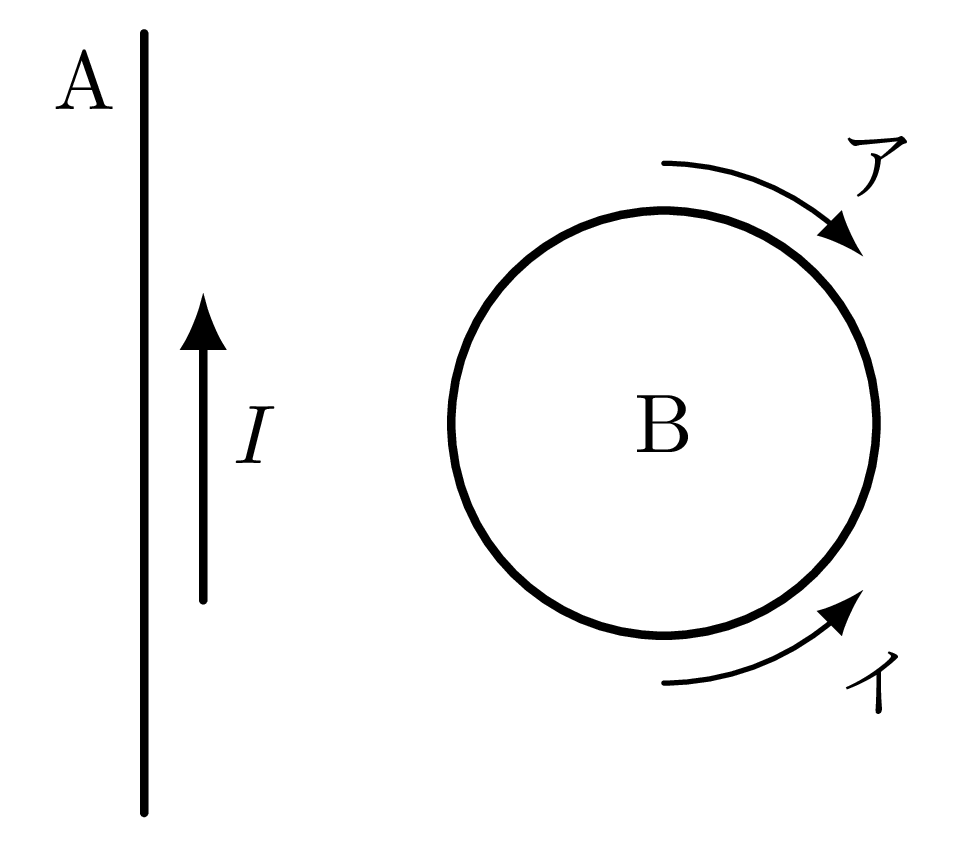
\includegraphics[keepaspectratio,width=38mm]{fig/n30_ex30_zu.png}
\end{zuright}
\end{reidai}

\begin{sisinE}
まず，直線電流が$\mathrm{B}$の位置につくる磁場の向きを右ねじの法則で決める．
次に，$\mathrm{B}$を貫く磁束が増えるか減るかを考え，その変化を打ち消す向きの磁場をつくる電流を答える．
\end{sisinE}

\Key{レンツの法則：誘導電流がつくる磁束は，外部の磁束の変化を打ち消す向き}

\begin{kaitou}
上向きの電流$I$は，その右側に{\gtfamily 紙面の表から裏の向き}の磁場をつくる．$\mathrm{B}$を貫く磁束はこの向きである．
\begin{komon}
\ko{1} $I$を増加させると，$\mathrm{B}$を裏向きに貫く磁束が増える．これを打ち消すには表向きの磁場が必要で，そのための電流は{\gtfamily 反時計回り}である．よって\AnaB{イ}\Ans
\ko{2} 導線から遠ざかると磁場が弱くなるので，$\mathrm{B}$を裏向きに貫く磁束が減る．これを打ち消す（補う）には裏向きの磁場が必要で，そのための電流は{\gtfamily 時計回り}である．よって\ ア\Ans
\end{komon}
\end{kaitou}
\end{reidaiunit}

\subsection{磁場を横切る導体棒の誘導起電力}

ファラデーの法則では，閉じたループを貫く磁束の変化を考えたが，実際には回路が閉じていなくても，{\gtfamily 導体棒が磁場を横切って運動するだけで，その導体棒に誘導起電力が発生する}．
この場合は，次のように考えて誘導起電力を求める．

\bsNeed{34mm}
\begin{matome}{導体棒の誘導起電力の求め方}
 \MARU{1}\ 導体棒が微小時間$dt$の間に掃く面積$dS$を計算する\\
 \MARU{2}\ その間に掃く磁束$d\varPhi=B\cdot dS$を求める\\
 \MARU{3}\ $dt$で割って，誘導起電力の大きさ$\left|\dfrac{d\varPhi}{dt}\right|$を求める
\end{matome}

\begin{zuright}{52mm}
\hspace{1zw}例として，磁束密度$B$の一様な磁場中を，磁場と棒の両方に垂直な向きに速さ$v$で動く長さ$l$の導体棒を考える．
この棒は$dt$の間に$v\,dt$だけ進むので，$dS=lv\,dt$の面積を掃き，$d\varPhi=vBl\,dt$の磁束を掃く．よって誘導起電力の大きさは
\AnaBD{V=vBl\U{V}}
である．
\zusep

\includegraphics[keepaspectratio,width=50mm]{text2_p71_fig1.png}
\end{zuright}

\begin{zuright}{50mm}
\hspace{1zw}導体棒が磁場を横切るとき誘導起電力が生じるのは，{\gtfamily 導体中の荷電粒子が棒と一緒に動いてローレンツ力を受ける}からである．
そこで，{\gtfamily 棒の上に正電荷を置き，それが棒と一緒に動くときに受けるローレンツ力の向きが誘導起電力の向き}である．
右図では，正電荷は$\mathrm{Q}\to\mathrm{P}$の向きに力を受けるので，棒の上に$\mathrm{Q}\to\mathrm{P}$の向きに大きさ$vBl$の電池ができたとみなせる（$\mathrm{P}$が高電位）．
\zusep

\includegraphics[keepaspectratio,width=48mm]{text2_p71_fig2.png}
\end{zuright}

% 加筆：原本 p72 の「参考」を本文に入れた（練習［109］の前提．再編案の指示）．
誘導起電力が生じる原因には次の2通りがあり，区別しておくとよい．
\begin{zuright}{44mm}
\noindent\MARU{1}\ {\gtfamily 磁束密度そのものが時間変化する場合}

\hspace{1zw}右図のように，ある円を貫く磁束$\varPhi$が時間変化すると，その円に沿って{\gtfamily 誘導電場}と呼ばれる電場$E$が生じる（導線が無くても空間に生じる）．
半径$r$の円に沿った誘導電場の大きさは$E=\dfrac{1}{2\pi r}\dfrac{d\varPhi}{dt}$であり，そこに1巻きの導線を置けば，一周で$V=E\cdot 2\pi r=\dfrac{d\varPhi}{dt}$の起電力になる．
静電場と違い，誘導電場の電気力線は閉じた輪になる．
\zusep

\includegraphics[keepaspectratio,width=42mm]{text2_p72_fig1.png}
\end{zuright}

\noindent\MARU{2}\ {\gtfamily 導体が磁場を横切って運動する場合}

導体中の荷電粒子が導体と一緒に動くことでローレンツ力を受け，一方向に押し流される．これは電池を置いたのと同じ効果なので，ローレンツ力のした仕事を電池の仕事と読み替えたものが誘導起電力である．
上の例では，$+q$の電荷が$\mathrm{Q}\to\mathrm{P}$に移る間にローレンツ力から$qvB\cdot l$の仕事をされるので，起電力$vBl$の電池があるのと同じになる（練習［102］）．
この場合は回路が閉じていなくても起電力が生じるので，上のまとめ枠の方法で大きさを求め，ローレンツ力で向きを決める．

\bsNeed{26mm}
\begin{matome}{導体棒に発生する誘導起電力の向き}
 \hspace{3mm} 導体棒の上に正電荷を置き，棒と一緒に動くときに受ける\AnaB{ローレンツ力の向き}に，大きさ$vBl$の電池が発生すると考える
\end{matome}

%%%%%%%%%%  例題31（原本の【例題33】）  %%%%%%%%%%%%%%%%%%%%
\bsNeed{56mm}
\begin{reidaiunit}
\begin{reidai}{一様な磁場中を回転する導体棒}
\begin{zuright}{40mm}
\hspace{1zw}図のように，長さ$r\U{m}$の導体棒$\mathrm{PQ}$を磁束密度$B\U{T}$の一様な磁場（紙面の表から裏の向き）に垂直に置き，その一端$\mathrm{P}$を中心にして，磁場に垂直な面内で角速度$\omega\U{rad/s}$で反時計回りに回転させる．導体棒に生じる誘導起電力について，以下の設問に答えよ．
\begin{komon}
\ko{1} 微小時間$dt$の間に導体棒が掃く面積を元にして，$\mathrm{PQ}$間に発生する誘導起電力の大きさを求めよ．
\ko{2} 導体棒と共に運動する正電荷が受ける力の向きを元にして，$\mathrm{P}$と$\mathrm{Q}$のいずれが高電位となるかを判定せよ．
\end{komon}
\zusep
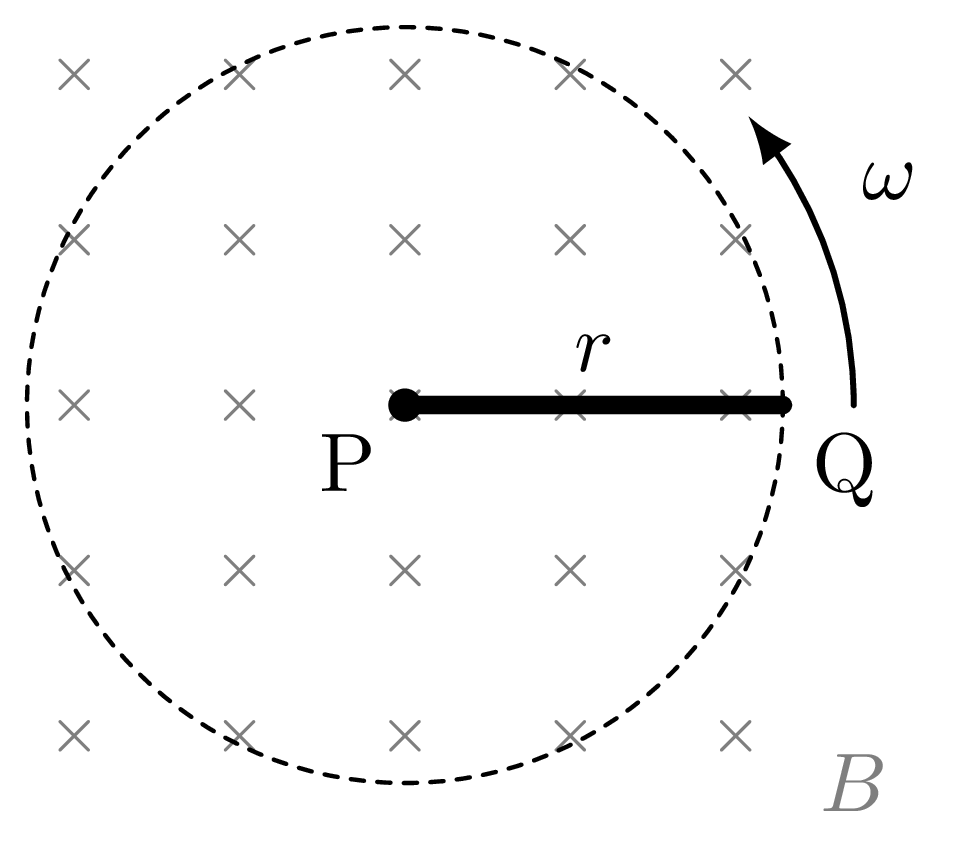
\includegraphics[keepaspectratio,width=38mm]{fig/n30_ex31_zu.png}
\end{zuright}
\end{reidai}

\begin{sisinE}
棒の各点の速さは$\mathrm{P}$からの距離に比例するので，$V=vBl$はそのままは使えない．
$dt$の間に棒は角$\omega\,dt$だけ回り，半径$r$，中心角$\omega\,dt$の扇形を掃く．この面積から$d\varPhi$を出せばよい．
\end{sisinE}

\Key{掃く面積$dS$から$d\varPhi=B\,dS$を求める\quad 向きは棒と共に動く正電荷が受けるローレンツ力の向き}

\begin{kaitou}
\begin{komon}
\ko{1} $dt$の間に掃く扇形の面積は$dS=\dfrac{1}{2}r^2\omega\,dt$なので，$d\varPhi=B\,dS$より
       \Ana{V=\frac{d\varPhi}{dt}=\frac{1}{2}B\omega r^2\U{V}\Ans}
       \begin{chuu}
       棒の中点の速さ$\dfrac{1}{2}r\omega$を使って$V=\bigl(\dfrac{1}{2}r\omega\bigr)Br$としても同じ結果になる（速さが位置に比例するので，平均の速さで計算してよい）．
       \end{chuu}
\ko{2} 図の瞬間，$\mathrm{Q}$付近の正電荷は上向きに動いている．磁場は裏向きなので，フレミングの左手の法則より正電荷は$\mathrm{Q}\to\mathrm{P}$の向きに力を受ける．正電荷が$\mathrm{P}$側に集まるので，{\gtfamily $\mathrm{P}$が高電位}である．\Ans
\end{komon}
\end{kaitou}
\end{reidaiunit}

\subsection{導体棒の運動と終端速度}

誘導電流が流れている導体棒は，磁場から電磁力を受ける．
レンツの法則から分かるように，{\gtfamily この電磁力は必ず導体棒の運動を妨げる向き}にはたらく．
したがって，一定の外力（重力など）を受けて磁場中を動く導体棒は，速くなるほど大きな逆向きの電磁力を受け，加速度はしだいに小さくなって，やがて一定の速度に近づく．これを{\gtfamily 終端速度}という．
終端速度では加速度が$0$なので，{\gtfamily 導体棒にはたらく力のつり合い}を立てれば求められる．

% 加筆：エネルギー収支（練習［103］の参考・例題32(5)）．
このとき，エネルギーの面では，外力が導体棒にした仕事（あるいは失われた力学的エネルギー）が，回路の抵抗でジュール熱として失われている．
終端速度に達したあとは，単位時間あたりの「外力の仕事」と「ジュール熱」が等しい．

\bsNeed{28mm}
\begin{matome}{磁場中を運動する導体棒}
 \hspace{3mm} 起電力$vBl$ → 誘導電流$I$ → 電磁力$IBl$（\AnaB{運動を妨げる向き}）の順に求め，運動方程式を立てる\\
 \hspace{3mm} 終端速度では力がつり合う．外力の仕事率＝ジュール熱の発生率
\end{matome}

%%%%%%%%%%  例題32（原本の【例題34】）  %%%%%%%%%%%%%%%%%%%%
\bsNeed{76mm}
\begin{reidaiunit}
\begin{reidai}{磁場中を落下していく導体棒}
\begin{zuright}{44mm}
\hspace{1zw}図のように，紙面に垂直（表から裏の向き）な磁束密度$B\U{T}$の一様な磁場中で，磁場に垂直な方向に水平に長さ$l\U{m}$の導線$\mathrm{EF}$を置き，その両端$\mathrm{E}$，$\mathrm{F}$から鉛直に導線$\mathrm{EC}$および$\mathrm{FD}$を立てる．それらの上に，$\mathrm{EF}$に沿って自由に上下に移動できる質量$m\U{kg}$，電気抵抗$R\U{\Omega}$の導体棒$\mathrm{K}$を取り付ける．他の部分の抵抗は無視できるものとする．導体棒$\mathrm{K}$を水平に保ちながら時刻$t=0$に初速度$0$で落下させる．$\mathrm{K}$は時刻$t\U{s}$に速さ$v\U{m/s}$になったものとする．$\mathrm{K}$と導線との間の摩擦は無視できるものとし，重力加速度の大きさを$g\U{m/s^2}$として以下の設問に答えよ．
\zusep
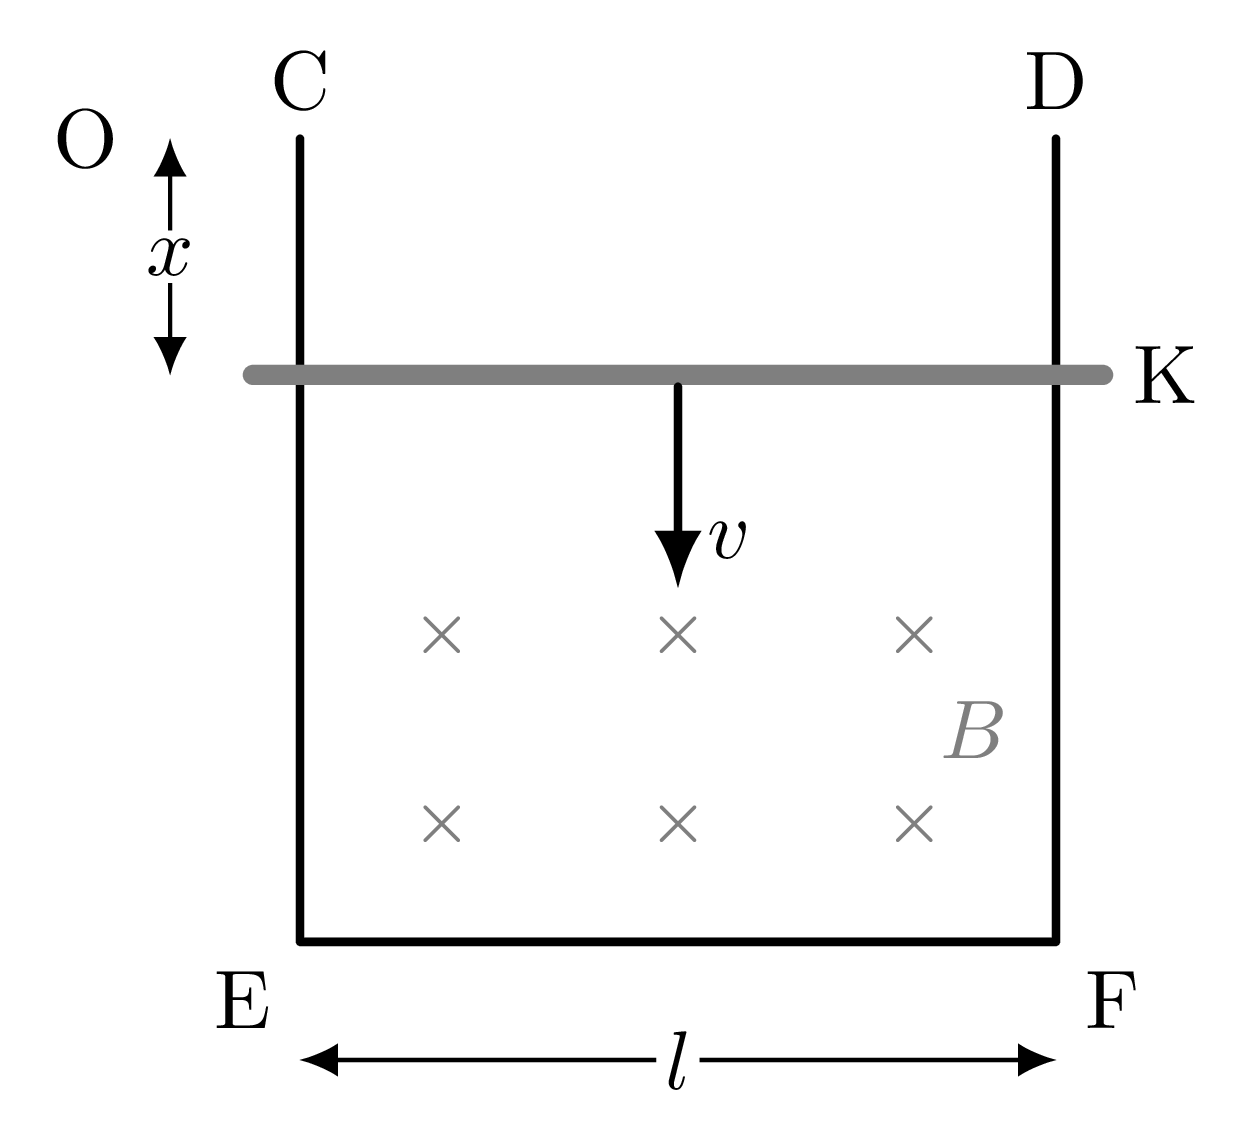
\includegraphics[keepaspectratio,width=42mm]{fig/n30_ex32_zu.png}
\end{zuright}
\begin{komon}
\ko{1} 時刻$t$において，導体棒$\mathrm{K}$に生じる誘導起電力を求めよ．
\ko{2} 時刻$t$において，この回路にはどちら向きにどれだけの大きさの電流が流れているか．
\ko{3} 時刻$t$における導体棒$\mathrm{K}$の運動方程式を求めよ．
\ko{4} 導体棒の終端速度を求め，このとき回路に流れる電流を求めよ．
\ko{5} (4)において，導体棒が単位時間あたりに失う力学的エネルギーと，導体棒で発生する単位時間あたりのジュール熱が等しいことを示せ．
\end{komon}
\end{reidai}

\begin{sisinE}
起電力$vBl$ → 電流$I=\dfrac{vBl}{R}$ → 電磁力$IBl$（上向き）の順に求め，下向きを正として運動方程式を立てる．
終端速度では加速度が$0$である．力の作用図を描いてから式を立てること．
\end{sisinE}

\Key{誘導起電力$vBl$\quad 電磁力$IBl$は運動を妨げる向き\quad 終端速度では力がつり合う}

\begin{kaitou}
\begin{komon}
\ko{1} \[V=vBl\U{V}\Ans\]
\ko{2} 正電荷が棒と共に下向きに動くと，磁場は裏向きなのでフレミングの左手の法則より$\mathrm{E}$側から$\mathrm{F}$側の向き（右向き）に力を受ける．よって$\mathrm{K}$の中を{\gtfamily 左から右}（$\mathrm{C}$側から$\mathrm{D}$側）に，大きさ
       \[I=\frac{vBl}{R}\U{A}\Ans\]
       の電流が流れる（回路全体では$\mathrm{K}\to\mathrm{D}\to\mathrm{F}\to\mathrm{E}\to\mathrm{C}\to\mathrm{K}$の向き）．
\ko{3} 右向きの電流は裏向きの磁場から上向きに$IBl$の電磁力を受ける（落下を妨げる向き）．加速度を$a$（下向き正）として
       \Ana{ma=mg-\frac{vB^2l^2}{R}\Ans}
\ko{4} $a=0$となる速さが終端速度$v_{\mathrm{f}}$なので
       \[v_{\mathrm{f}}=\frac{mgR}{B^2l^2}\U{m/s}\Ans\]
       このとき
       \[I_{\mathrm{f}}=\frac{v_{\mathrm{f}}Bl}{R}=\frac{mg}{Bl}\U{A}\Ans\]
       （電磁力$I_{\mathrm{f}}Bl$が重力$mg$とつり合っている．）
\ko{5} 終端速度では運動エネルギーが変わらないので，単位時間あたりに失う力学的エネルギーは位置エネルギーの減少$mgv_{\mathrm{f}}=\dfrac{m^2g^2R}{B^2l^2}$である．一方，ジュール熱は$I_{\mathrm{f}}^2R=\dfrac{m^2g^2}{B^2l^2}R$．両者は等しい．\Ans
\end{komon}
\end{kaitou}
\end{reidaiunit}

\subsection{自己誘導とコイルのエネルギー}

\begin{zuright}{50mm}
\hspace{1zw}コイルに流れる電流が増加しようとする場合を考える．コイルを流れる電流がつくる磁場が増加するので，コイルには電流とは逆向きの誘導起電力が生じ，電流の増加を妨げようとする．この現象を{\gtfamily 自己誘導}と呼ぶ．
\zusep

\includegraphics[keepaspectratio,width=48mm]{text2_p74_fig1.png}
\end{zuright}
コイルを貫く磁束はコイルの電流$I$に比例し，誘導起電力は磁束の時間変化率に比例するので，比例定数を$L$として，自己誘導起電力の大きさは$L\left|\dfrac{dI}{dt}\right|$と書ける．
$L$を{\gtfamily 自己インダクタンス}といい，コイルの形状（巻き数・長さ・断面積）と中の物質で決まる．単位は$\U{H}$（ヘンリー）である．
流れている電流の向きを正とすると，自己誘導起電力は
\AnaBD{V=-L\frac{dI}{dt}\U{V}}
である．電流が増加するとき（$\dfrac{dI}{dt}>0$）は電流と逆向き，減少するとき（$\dfrac{dI}{dt}<0$）は電流と同じ向きになる．
{\gtfamily コイルは自分に流れる電流の変化を妨げる}素子である．

% 誤植訂正：旧 physics_ch39.tex のまとめ枠は「V=--L dI/dt」だった．
\bsNeed{26mm}
\begin{matome}{自己誘導}
 \hspace{3mm} コイルを流れる電流$I$が変化するとき，電流の向きを正として$V=-L\dfrac{dI}{dt}\U{V}$の自己誘導起電力が生じる\\
 \hspace{3mm} （電流の変化を妨げる向き）
\end{matome}

コンデンサーに電荷を与えると静電エネルギーが蓄えられたのと同様に，自己インダクタンス$L$のコイルに電流$I$を流すと，コイルの内部の磁場という形で
\AnaBD{U=\frac{1}{2}LI^2\U{J}}
のエネルギーが蓄えられる．
導出：電流が$i$のとき，自己誘導起電力$L\dfrac{di}{dt}$に逆らって電流を流し込むには，外から同じ大きさの電圧をかけなければならない．$dt$の間に送り込む電荷は$i\,dt$なので，その仕事は$dW=i\,dt\cdot L\dfrac{di}{dt}=Li\,di$．$i=0$から$I$まで足して$W=\displaystyle\int_0^ILi\,di=\dfrac{1}{2}LI^2$となる．

%%%%%%%%%%  例題33（原本の【例題35】）  %%%%%%%%%%%%%%%%%%%%
\bsNeed{60mm}
\begin{reidaiunit}
\begin{reidai}{自己インダクタンス}
\begin{zuright}{56mm}
\hspace{1zw}図のように，断面積$S\U{m^2}$，長さ$l\U{m}$，単位長さあたりの巻き数$n_0\U{/m}$のコイルを用意する．今，このコイルに図の向きに電流$I\U{A}$を流す．この空間の透磁率を$\mu_0\U{Wb^2/N\cdot m^2}$として以下の設問に答えよ．
\begin{komon}
\ko{1} このコイルを貫く磁束$\varPhi\U{Wb}$およびその向きを求めよ．
\ko{2} このコイルに流す電流を微小時間$\varDelta t$の間に$\varDelta I$だけ増加させるとき，コイルにはどんな向きの誘導起電力が発生するか．
\ko{3} (2)について，誘導起電力の大きさを求めよ．
\ko{4} このコイルの自己インダクタンスを求めよ．
\end{komon}
\zusep
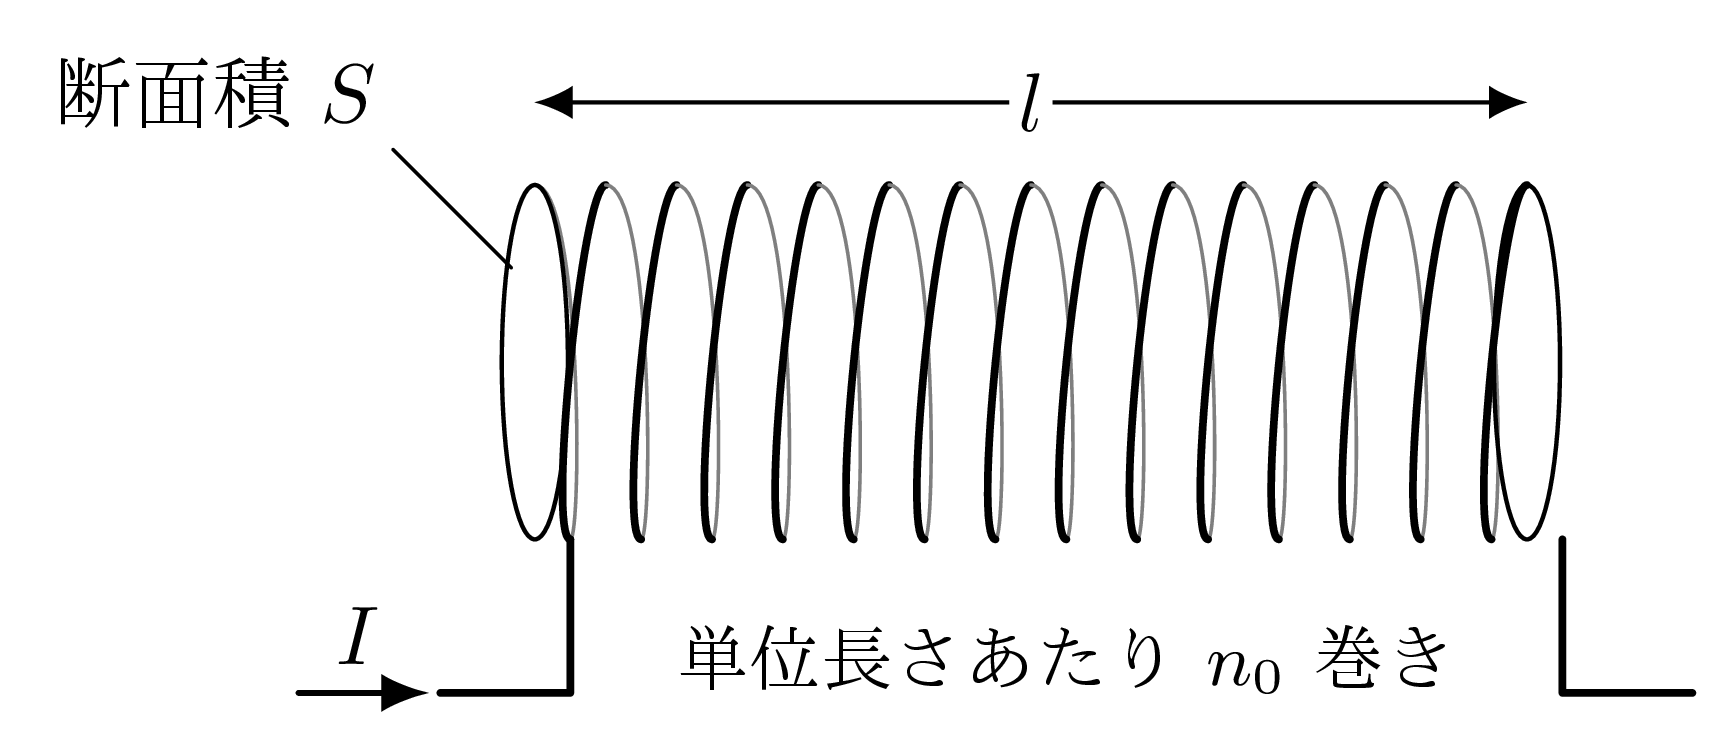
\includegraphics[keepaspectratio,width=54mm]{fig/n30_ex33_zu.png}
\end{zuright}
\end{reidai}

\begin{sisinE}
コイル内部の磁場$H=n_0I$ → 磁束$\varPhi=\mu_0HS$ → ファラデーの法則．
全巻き数は$N=n_0l$であることに注意（$N$倍を忘れない）．
\end{sisinE}

\Key{ファラデーの電磁誘導の法則$V=-N\dfrac{d\varPhi}{dt}$\quad 自己誘導起電力$V=-L\dfrac{dI}{dt}$}

\begin{kaitou}
\begin{komon}
\ko{1} 内部の磁場は$H=n_0I$なので
       \[\varPhi=\mu_0n_0IS\U{Wb}\Ans\]
       向きはコイルの軸に平行で，電流の向きに右ねじを回したときにねじが進む向き（図では右向き）．\Ans
\ko{2} 磁束の増加を打ち消す向き，すなわち{\gtfamily 流している電流と逆向き}の電流を流そうとする向きに生じる．\Ans
\ko{3} 1巻きあたりの磁束の変化は$\varDelta\varPhi=\mu_0n_0S\varDelta I$，巻き数は$N=n_0l$なので
       \Ana{V=N\frac{\varDelta\varPhi}{\varDelta t}=\mu_0n_0^2Sl\frac{\varDelta I}{\varDelta t}\U{V}\Ans}
\ko{4} $V=L\dfrac{\varDelta I}{\varDelta t}$と比べて
       \[L=\mu_0n_0^2Sl\U{H}\Ans\]
       （巻き数の2乗と体積$Sl$に比例する．）
\end{komon}
\end{kaitou}
\end{reidaiunit}

\subsection{相互誘導}

\begin{center}

\includegraphics[keepaspectratio,width=90mm]{text2_p77_fig1.png}
\end{center}
自己誘導ではコイルが自分自身を貫く磁束の変化で生じる起電力を考えたが，上図のように軸をそろえて置いた2つのコイルの間でも同様の現象が起こる．
一方のコイル（{\gtfamily 1次コイル}）の電流$I_1$を変化させると，もう一方のコイル（{\gtfamily 2次コイル}）に誘導起電力が生じる．これを{\gtfamily 相互誘導}という．
2次コイルを貫く磁束は$I_1$に比例するので，2次コイルの誘導起電力の大きさは比例定数を$M$として$M\left|\dfrac{dI_1}{dt}\right|$と書ける．
% 誤植訂正：旧 physics_ch39.tex は「M dΦ/dt」になっていた．
$M$を{\gtfamily 相互インダクタンス}といい，2つのコイルの形状と配置で決まる．単位は$\U{H}$である．

相互誘導起電力の向きは2つのコイルの配置・巻き方で決まるので，次の手順で決める．
\begin{description}
\item[\MARU{1}] 1次コイルの電流$I_1$がつくる磁場の向きを考える．
\item[\MARU{2}] \MARU{1}と同じ向きの磁場をつくる2次コイルの電流の向きを正とする．
\item[\MARU{3}] 正の向きに電流を流そうとする起電力を正とする（上図では$\mathrm{c}\to\mathrm{d}$）．
\end{description}
こうして向きを決めると，2次コイルの起電力は
\AnaBD{V_2=-M\frac{dI_1}{dt}\U{V}}
となる．

\bsNeed{26mm}
\begin{matome}{相互誘導}
 \hspace{3mm} 1次コイルの電流$I_1$が変化するとき，2次コイルに$V_2=-M\dfrac{dI_1}{dt}$の相互誘導起電力が生じる\\
 \hspace{3mm} （正の向きは，1次コイルの磁場と同じ向きの磁場をつくる電流の向き）
\end{matome}

%%%%%%%%%%  例題34（原本の【例題37】）  %%%%%%%%%%%%%%%%%%%%
\bsNeed{76mm}
\begin{reidaiunit}
\begin{reidai}{相互誘導}
\begin{zuright}{56mm}
\hspace{1zw}図のように，鉄心に同じ向きに巻いた2つのコイル$\mathrm{A}$，$\mathrm{B}$がある（端子$\mathrm{a}$と$\mathrm{c}$，$\mathrm{b}$と$\mathrm{d}$がそれぞれ同じ側にある）．コイル$\mathrm{A}$に可変電源を取り付けてスイッチ$\mathrm{S}$を閉じ，可変電源を操作して，コイル$\mathrm{A}$に$\mathrm{a}$から入って$\mathrm{b}$へ抜ける向きに流す電流$I$を変化させる．以下の問いに答えよ．
\zusep
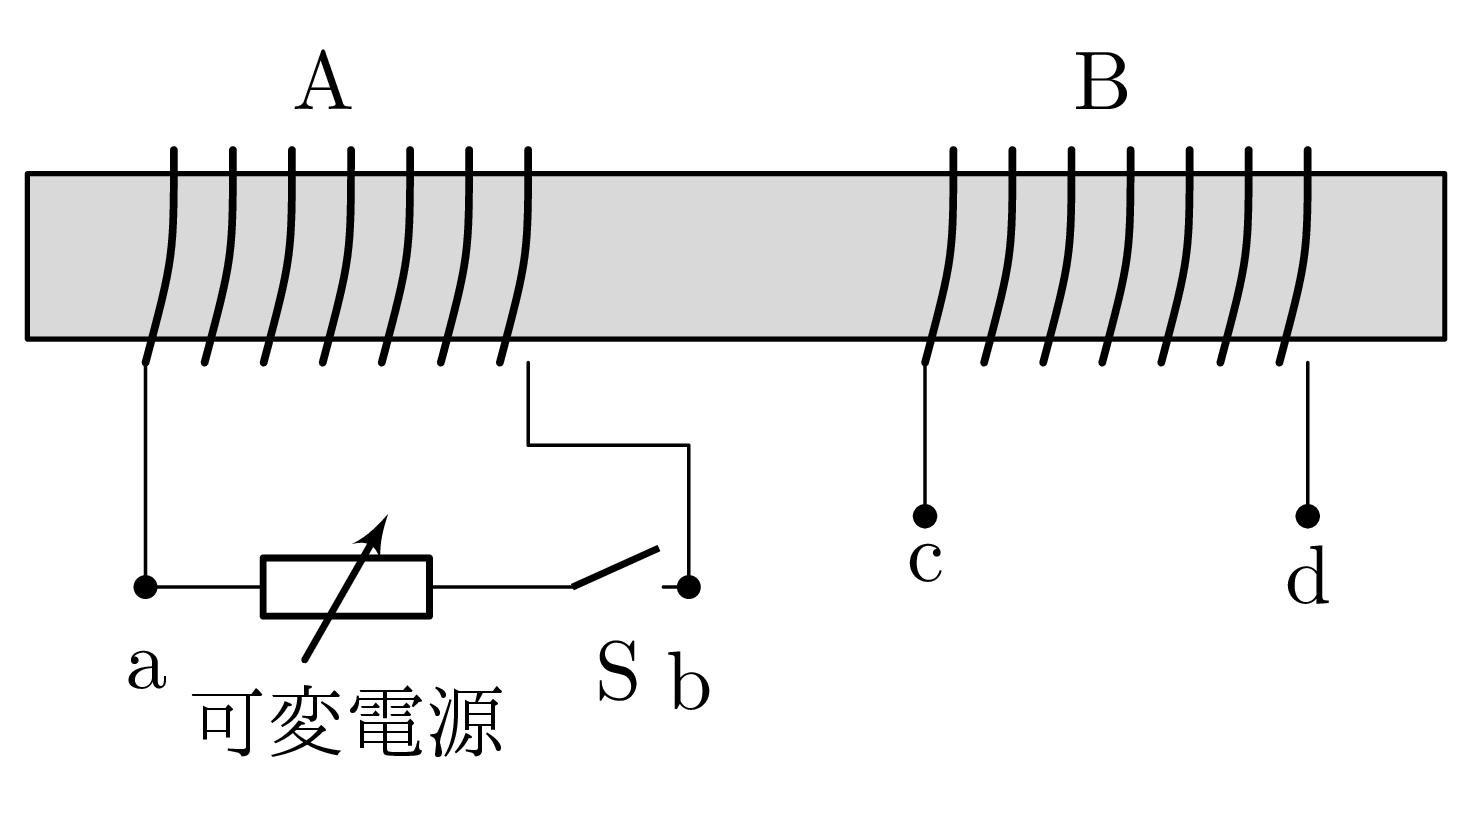
\includegraphics[keepaspectratio,width=54mm]{fig/n30_ex34_zu.png}
\end{zuright}
\begin{komon}
\ko{1} コイル$\mathrm{A}$に流れる電流を増加させるとき，高電位となるのは$\mathrm{a}$と$\mathrm{b}$のどちらか．
\ko{2} そのとき，コイル$\mathrm{B}$に相互誘導起電力が生じるが，高電位となるのは$\mathrm{c}$と$\mathrm{d}$のどちらか．
\ko{3} 今，コイル$\mathrm{A}$の可変電源を操作して，$\mathrm{A}$に流れる電流を$2\U{A/s}$の割合で増加させたところ，図の$\mathrm{ab}$間には$10\U{V}$の電位差が，$\mathrm{cd}$間には$6\U{V}$の電位差が生じた．これを元に，コイル$\mathrm{A}$の自己インダクタンス$L\U{H}$およびコイル$\mathrm{A}$，$\mathrm{B}$間の相互インダクタンス$M\U{H}$を求めよ．
\ko{4} また，可変電源の操作によりコイル$\mathrm{A}$に定常的に一定の電流が流れるようになったあと，スイッチ$\mathrm{S}$を開いた．開いた直後は$\mathrm{a}$と$\mathrm{b}$のいずれが高電位となるか．
\ko{5} (4)のとき，$\mathrm{c}$と$\mathrm{d}$はどちらが高電位となるか．
\end{komon}
\end{reidai}

\begin{sisinE}
コイル$\mathrm{A}$を「電流の変化を妨げる電池」と考える．電流が増えるときは電流を押し戻す向き（抵抗の電圧降下と同じく，電流が入る側が高電位），減るときは電流を押し出す向きの電池になる．
コイル$\mathrm{B}$は$\mathrm{A}$と同じ向きに巻かれ，同じ磁束が貫くので，$\mathrm{c}$，$\mathrm{d}$の電位の関係は$\mathrm{a}$，$\mathrm{b}$と同じになる．
\end{sisinE}

\Key{自己誘導$-L\dfrac{dI}{dt}$\quad 相互誘導$-M\dfrac{dI_1}{dt}$\quad いずれも磁束の変化を妨げる向き}

\begin{kaitou}
\begin{komon}
\ko{1} 電流の増加を妨げる向き（$\mathrm{b}\to\mathrm{a}$の向きに電流を流そうとする向き）に起電力が生じる．コイル$\mathrm{A}$は$\mathrm{a}$から入る電流を押し戻す電池としてはたらくので，{\gtfamily $\mathrm{a}$}が高電位．\Ans
\ko{2} $\mathrm{B}$を貫く磁束も$\mathrm{A}$と同じように増えるので，$\mathrm{B}$にも$\mathrm{A}$と同じ向き（$\mathrm{d}\to\mathrm{c}$に電流を流そうとする向き）の起電力が生じる．$\mathrm{B}$は開いているので電流は流れず，{\gtfamily $\mathrm{c}$}が高電位になる．\Ans
\ko{3} $V_{\mathrm{ab}}=L\dfrac{dI}{dt}$，$V_{\mathrm{cd}}=M\dfrac{dI}{dt}$より
       \Ana{L=\frac{10}{2}=5\U{H},\qquad M=\frac{6}{2}=3\U{H}\Ans}
\ko{4} 電流が急に減少するので，それを妨げる向き（電流を$\mathrm{a}\to\mathrm{b}$の向きに流し続けようとする向き）に起電力が生じる．コイルは$\mathrm{b}$から電流を押し出す電池としてはたらくので，{\gtfamily $\mathrm{b}$}が高電位．\Ans
\ko{5} $\mathrm{B}$も同様に{\gtfamily $\mathrm{d}$}が高電位．\Ans
       \begin{chuu}
       スイッチを開くと電流は非常に短い時間で$0$になるので，$\left|\dfrac{dI}{dt}\right|$が大きく，大きな起電力が生じる（スイッチに火花が飛ぶことがある）．
       \end{chuu}
\end{komon}
\end{kaitou}
\end{reidaiunit}

% 加筆：変圧器（練習［106］の前提．再編案「変圧器の巻数比・理想的な電力保存を練習の前に」）．
\subsection{変圧器}

鉄心に1次コイル（巻き数$N_1$）と2次コイル（巻き数$N_2$）を巻いたものを{\gtfamily 変圧器（トランス）}という．
鉄心は磁束を閉じ込めるので，鉄心がどのような形でも，{\gtfamily 両方のコイルを同じ磁束$\varPhi$が貫く}．
1巻きあたりの起電力はどちらも$\dfrac{d\varPhi}{dt}$なので，2つのコイルの電圧は巻き数に比例する：
\AnaBD{V_1:V_2=N_1:N_2}
1次コイルに交流電圧をかければ，2次コイルに巻き数比に応じた交流電圧が得られる（電圧を変える装置なので変圧器という．交流は第31回）．
エネルギーの損失が無い理想的な変圧器では，1次側に供給される電力と2次側で取り出される電力は等しく，$V_1I_1=V_2I_2$が成り立つ．

\newpage

%%%%%%%%%%%%%%%%%%%%  練習問題  %%%%%%%%%%%%%%%%%%%%
% 第29回の［98］に続く．
\setcounter{qno}{98}

\filbreak
\Rank{A問題}

% A問題の統合（再編案の「A2→1」）：旧㊳[64]（(1)(2)）と旧㊴[71]（(1)〜(3)）を1題にまとめた．
%   (3)〜(5) が旧㊴[71] の(1)〜(3)．
\Mon{基本公式の確認}

\hspace{1zw}以下の設問に答えよ．
\begin{komon}
\ko{1} 次の\MARU{1}から\MARU{4}の操作を行うと，図の端子$\mathrm{a}$，$\mathrm{b}$のどちらの方が高電位となるか．
\end{komon}
\begin{center}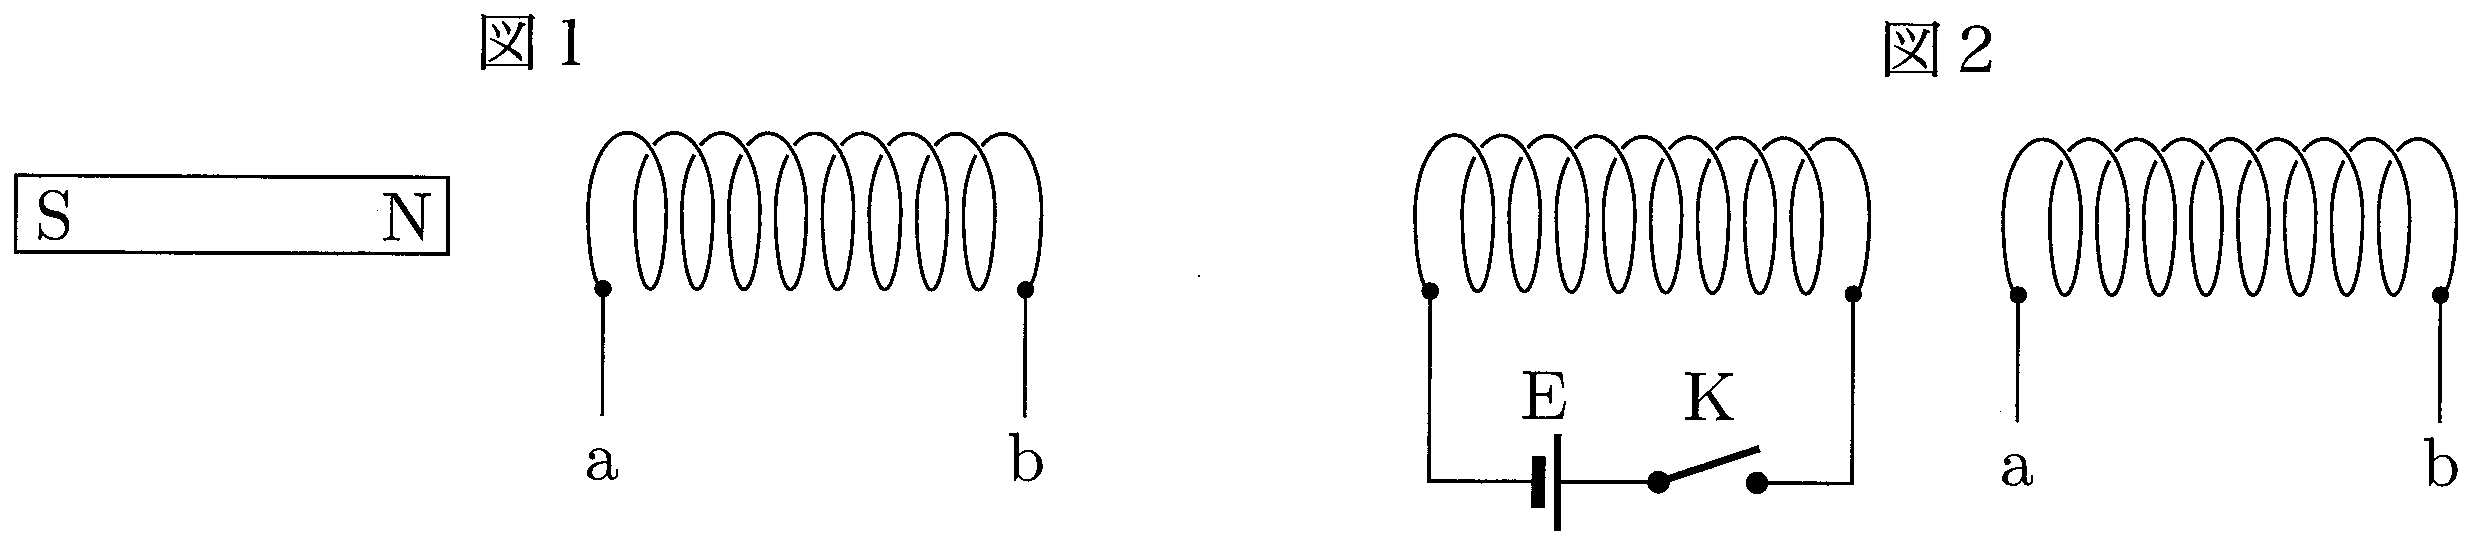
\includegraphics[keepaspectratio,width=150mm]{fig/n30_p99_zu1.png}\end{center}
\hspace{3zw}\MARU{1}\ 図1で磁石をコイルに近づける\qquad\MARU{2}\ 図1でコイルを下方へ動かす\\
\hspace*{3zw}\MARU{3}\ 図2でスイッチを入れた直後\qquad\MARU{4}\ 図2でスイッチを入れて十分時間が経った後
\begin{komon}
\ko{2} 断面積$3.0\times 10^{-4}\U{m^2}$，巻数$500$回のコイルの断面を貫く磁束密度が，$2.0\times 10^{-2}\U{s}$間に一定の割合で$4.0\times 10^{-2}\U{Wb/m^2}$だけ変化した．このときコイルに生じる誘導起電力の大きさは何$\U{V}$か．
\ko{3} 自己インダクタンス$30\U{H}$のコイルに流れる電流を，一定の増加率で$2.0\U{s}$間に$0.10\U{A}$だけ変化させた．コイルに生じる自己誘導起電力の大きさは何$\U{V}$か．
\end{komon}
\begin{zuright}{50mm}
\begin{komon}
\ko{4} 2個の円形コイル$\mathrm{A}$，$\mathrm{B}$を右図のように中心軸を一致させて重ねた．$\mathrm{A}$には電池とスイッチ$\mathrm{S}$をつける．もともと二つのコイルのいずれにも電流は流れていなかった．$\mathrm{S}$を閉じた瞬間にコイル$\mathrm{B}$を流れる電流の向きは$\mathrm{a}$，$\mathrm{b}$のいずれか．
\end{komon}
\zusep
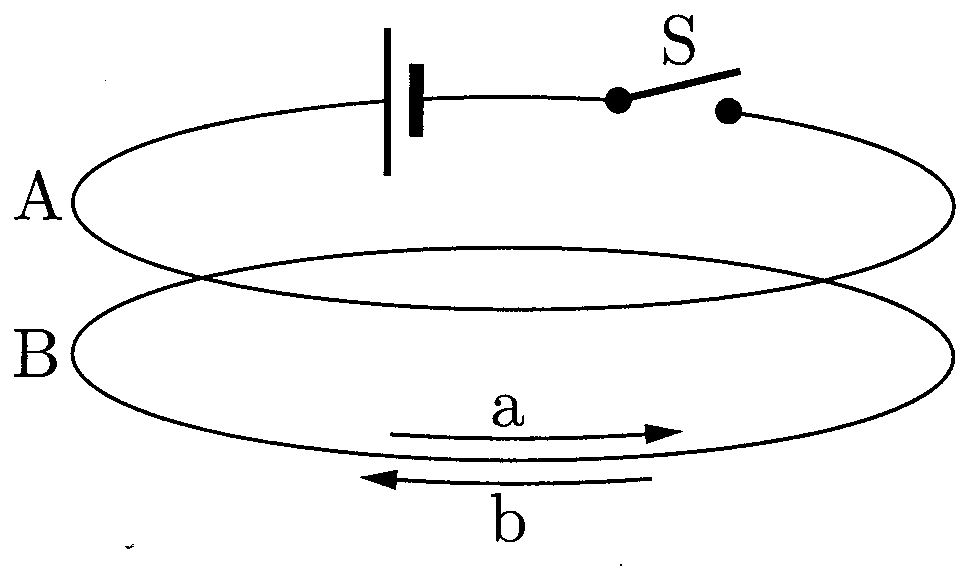
\includegraphics[keepaspectratio,width=46mm]{fig/n30_p99_zu2.png}
\end{zuright}
\begin{zuright}{56mm}
\begin{komon}
\ko{5} 右図の回路において，可変抵抗を調節して，コイル1に流れる電流$I$を一定の増加率で$0.50\U{s}$間に$2.0\U{A}$だけ変化させた．コイル1とコイル2の相互インダクタンスが$4.0\U{H}$であるとき，コイル2に生じる相互誘導起電力の大きさは何$\U{V}$か．
\end{komon}
\zusep
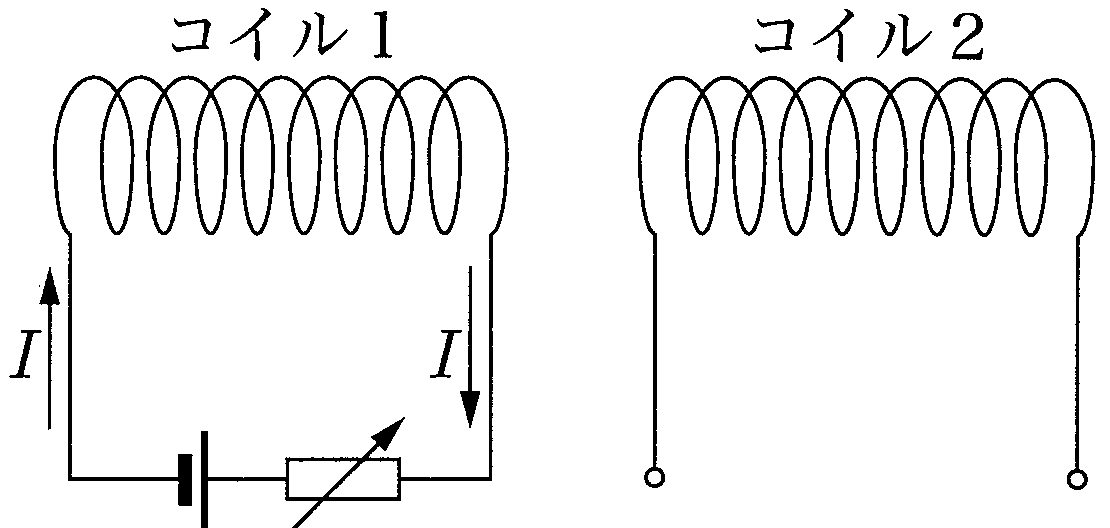
\includegraphics[keepaspectratio,width=52mm]{fig/n30_p99_zu3.png}
\end{zuright}

\filbreak
\Rank{B問題}

\Mon{回路に生じる誘導起電力}

\hspace{1zw}図1のような回路を貫く磁束$\varPhi\U{Wb}$が図2のように変化するとき，回路に生じる誘導起電力$V\U{V}$の時間変化を図に示せ．ただし誘導電流の向きが反時計回りとなるときを正として答えよ．
\begin{center}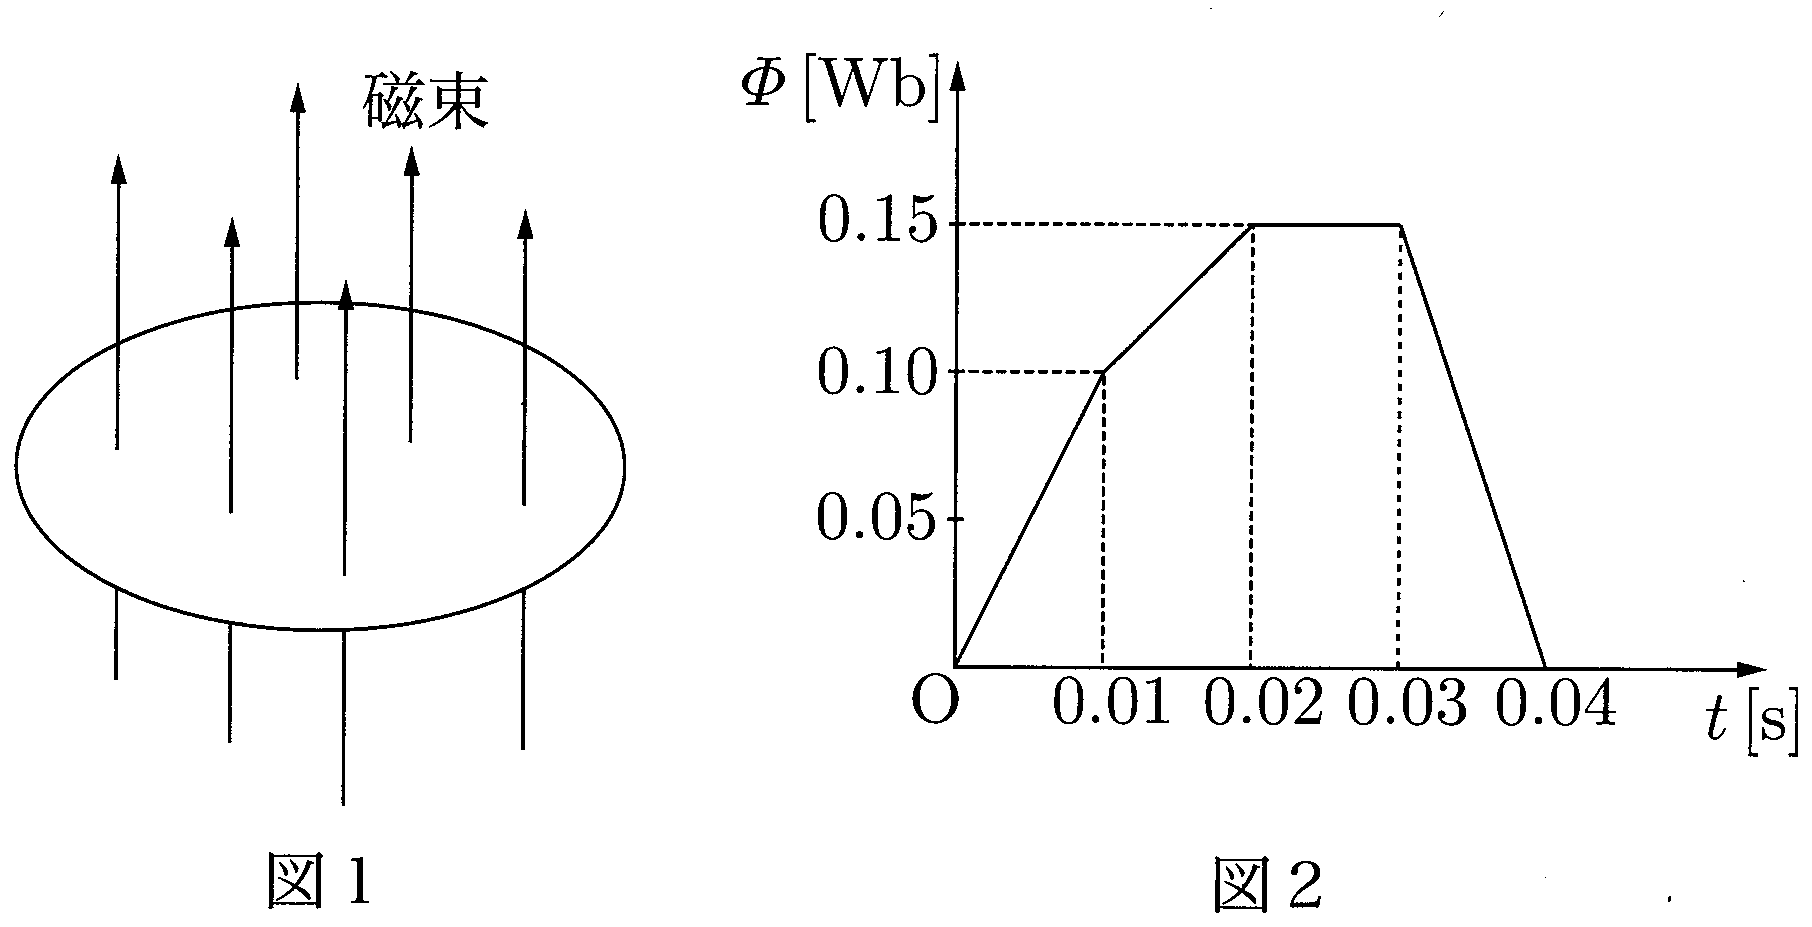
\includegraphics[keepaspectratio,width=96mm]{fig/n30_p100_zu.png}\end{center}

\Mon{矩形コイルの電磁誘導}

\begin{zuright}{62mm}
\hspace{1zw}右図のように間隔$l\U{m}$の平行導線$\mathrm{XX}^\prime$，$\mathrm{YY}^\prime$を水平面内におき，$\mathrm{XY}$間に抵抗値$R\U{\Omega}$の抵抗$\mathrm{R}$をつなぐ．この空間には回路の面に対して図のように垂直上向きに一様な磁束密度$B\U{Wb/m^2}$の磁場がかけられている．今，この矩形回路上に導体棒$\mathrm{PQ}$を水平導線に対して垂直となるように置き，これに外力を加えて一定の速さ$v\U{m/s}$で$\mathrm{XY}$に近づける向きに動かす．以下の問いに答えよ．
\zusep
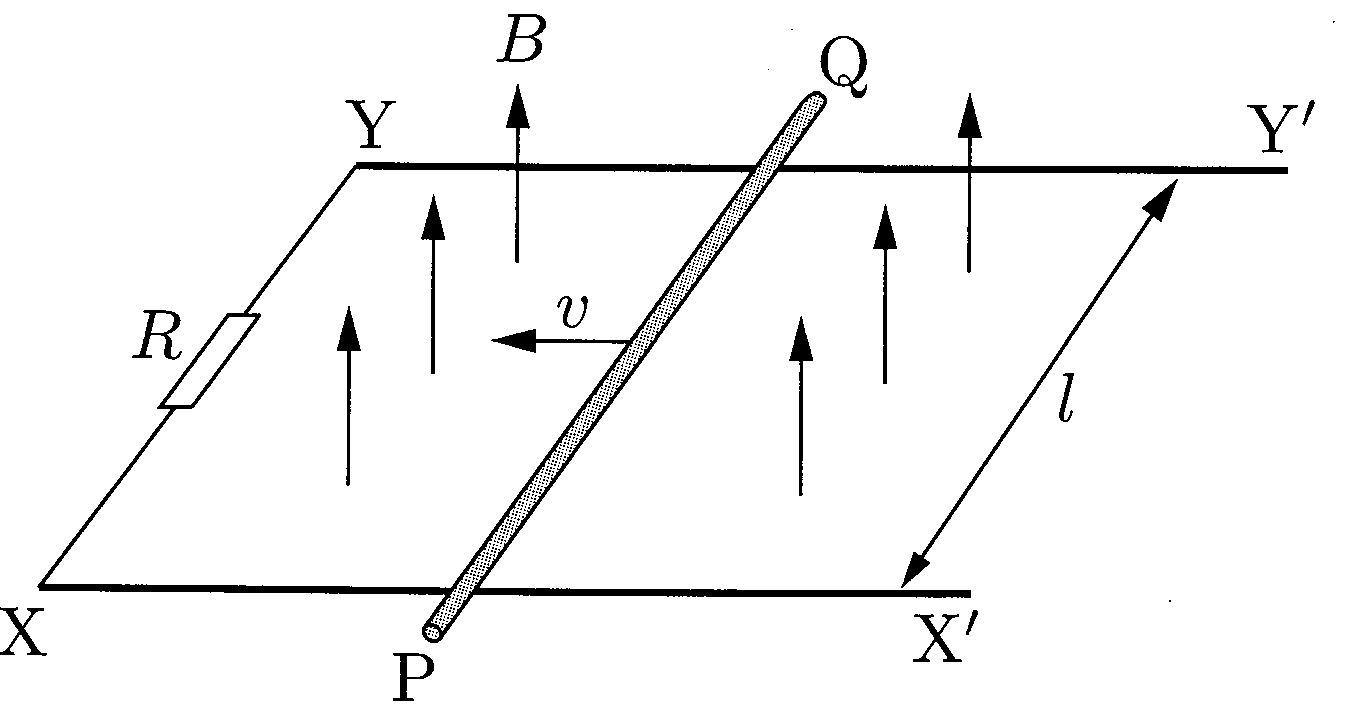
\includegraphics[keepaspectratio,width=60mm]{fig/n30_p101_zu.png}
\end{zuright}
\begin{komon}
\ko{1} 導体棒$\mathrm{PQ}$に生じる誘導起電力の大きさおよび向きを求めよ．
\ko{2} この回路に生じる誘導電流の大きさおよび向きを求めよ．
\ko{3} 導体棒$\mathrm{PQ}$を一定速度で動かすために加えている外力の大きさおよび向きを求めよ．
\end{komon}

\Mon{ローレンツ力と電磁誘導}

\begin{zuright}{50mm}
\hspace{1zw}次の\framebox[4zw]{\rule{0pt}{1.1zw}1}から\framebox[4zw]{\rule{0pt}{1.1zw}5}に当てはまる適当な語句および数値を入れよ．
\par
\hspace{1zw}右図のように，磁束密度$B\U{Wb/m^2}$の一様な磁場中に，長さ$l\U{m}$の導体棒$\mathrm{PQ}$が磁場に対して垂直に置かれている．今，導体棒$\mathrm{PQ}$をその長さの方向と磁場に対して垂直に速さ$v\U{m/s}$で動かす．
\zusep
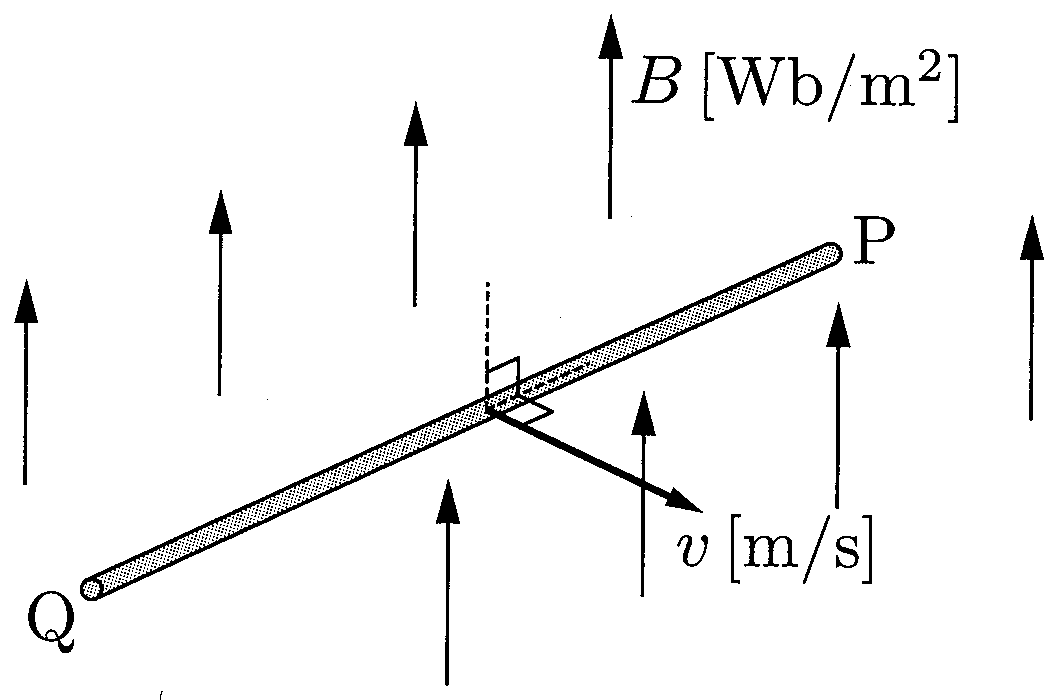
\includegraphics[keepaspectratio,width=48mm]{fig/n30_p102_zu.png}
\end{zuright}
電子の電荷を$-e\U{C}$とすると，このとき導体棒$\mathrm{PQ}$内の電子は導体棒と共に運動することにより，磁場から\framebox[4zw]{\rule{0pt}{1.1zw}1}の向きに大きさ$f=$\framebox[4zw]{\rule{0pt}{1.1zw}2}のローレンツ力を受けることになる．これは，導体棒$\mathrm{PQ}$内に\framebox[4zw]{\rule{0pt}{1.1zw}3}の向きに，大きさ$E=$\framebox[4zw]{\rule{0pt}{1.1zw}4}の一様電場が生じているときに受ける力と同じであるから，このように導体棒$\mathrm{PQ}$が磁場に対して垂直に移動するということは，導体棒内に電場が生じたのと同じ効果を持つ．よってこのことより，導体棒$\mathrm{PQ}$の両端間の電位差は$V=E\cdot l=$\framebox[4zw]{\rule{0pt}{1.1zw}5}であると求めることができ，結局，本問のように磁場中を導体棒が横切る場合に生じる誘導起電力はローレンツ力により生じていることが分かる．

\Mon[\Sitei]{終端速度}

\begin{zuright}{60mm}
\hspace{1zw}鉛直下向きの一様な磁束密度$B\U{Wb/m^2}$の磁場中に，金属レール$\mathrm{XY}$，$\mathrm{X}^\prime\mathrm{Y}^\prime$を水平かつ$l\U{m}$の間隔で平行に固定し，その上に質量$m\U{kg}$の金属棒を乗せ，$\mathrm{XX}^\prime$に抵抗値$R\U{\Omega}$の抵抗をつないだ．$\mathrm{XY}$にはスイッチがあり，内部抵抗の無視できる起電力$E\U{V}$の電池に接続することができるようになっている．$R\U{\Omega}$の抵抗以外の電気抵抗は無視してよいものとし，金属棒はレールに垂直を保ったまま滑らかに動けるものとする．右向きを速度・加速度の正の向きとして，以下の設問に答えよ．
\zusep
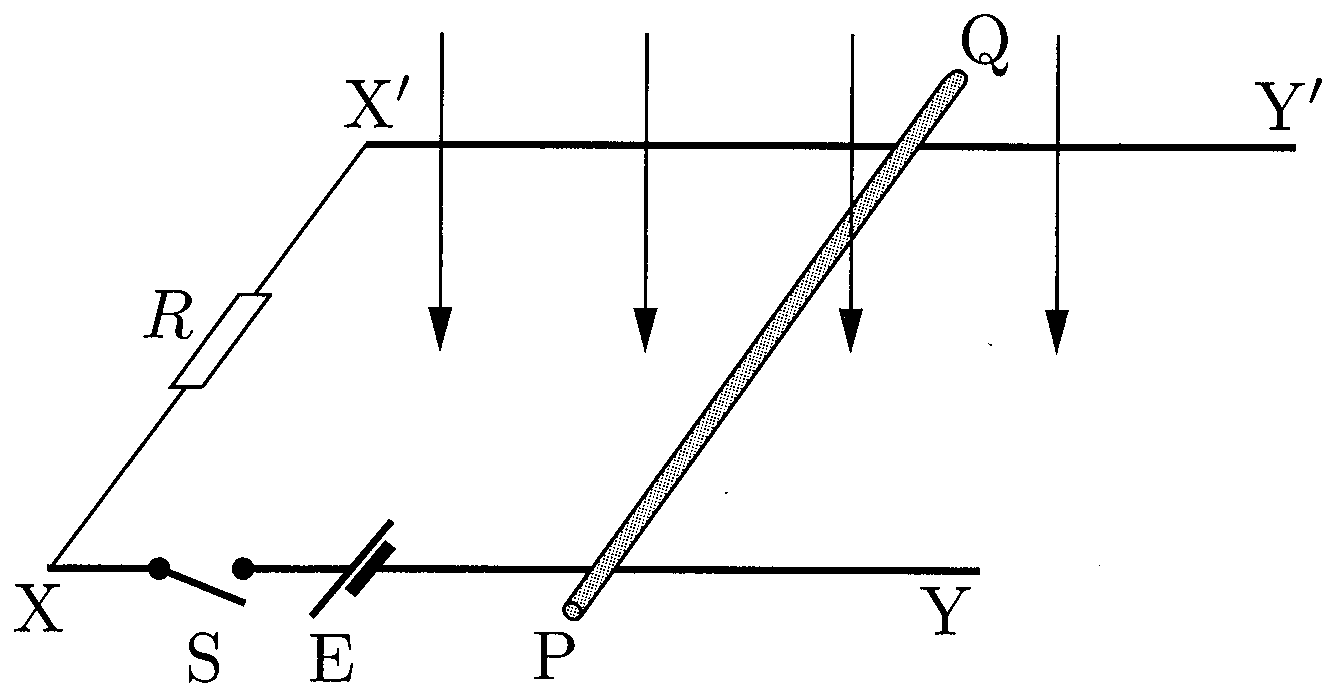
\includegraphics[keepaspectratio,width=58mm]{fig/n30_p103_zu.png}
\end{zuright}
\begin{komon}
\ko{1} スイッチ$\mathrm{S}$を入れると棒が動き始める．棒の速度は変化していくが，その速度がちょうど$v\U{m/s}$になったときについて，回路に流れる電流$I\U{A}$を$v$を用いて表し，さらに導体棒の加速度を$a\U{m/s^2}$として，導体棒の運動方程式を示せ．ただし，電流は上面から見て時計回りに流れるときを正にとって答えよ．
\ko{2} スイッチ$\mathrm{S}$を入れてから十分時間が経過したときの導体棒の速度（終端速度）を求めよ．またこのとき，抵抗での消費電力はいくらか．
\end{komon}

\Mon[\Sitei]{回路の運動}

\hspace{1zw}下図のように幅$L\U{m}$の領域に紙の表から裏に向かって紙面に対して垂直な一様な磁束密度$B\U{Wb/m^2}$の磁場がある．紙面でこの磁場に向かって，$\mathrm{AB}=a\U{m}$，$\mathrm{BC}=b\U{m}$の長方形回路（$L>b$，全抵抗$R\U{\Omega}$）が速さ$v\U{m/s}$で近づく．$\mathrm{CD}$と$\mathrm{EF}$とが一致する時刻を$0\U{s}$とする．時刻$t\U{s}$において，この回路に生じる誘導電流$I(t)\U{A}$を求めよ．ただし，反時計回りに電流が流れる場合を正として答えよ．
\begin{center}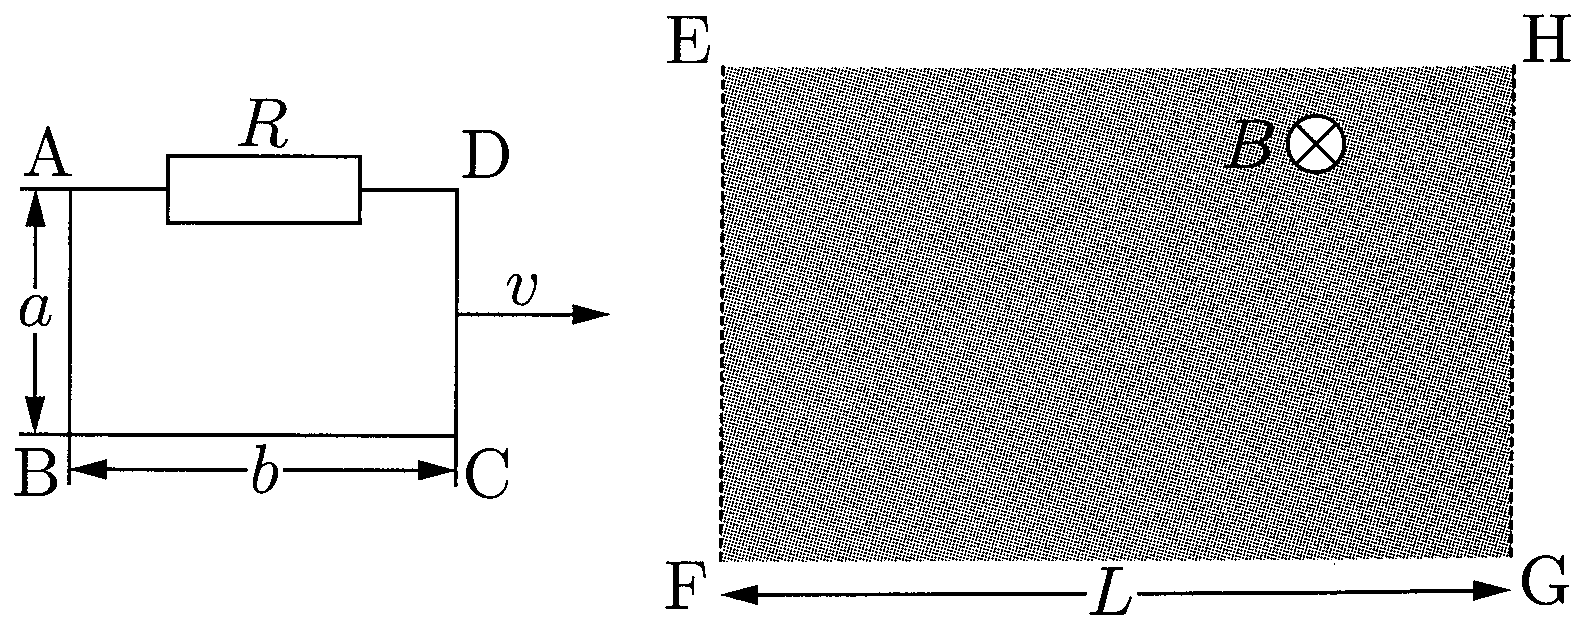
\includegraphics[keepaspectratio,width=100mm]{fig/n30_p104_zu.png}\end{center}

\Mon[\Sitei]{相互誘導起電力}

\hspace{1zw}図1のようなコイル1とコイル2が鉄心に巻いてあり，コイル1，2間の相互インダクタンスは$0.010\U{H}$である．コイル1の$\mathrm{a}\to\mathrm{b}$の矢印の向きに図2のような電流$I\U{A}$を流したとき，コイル2に生じる誘導起電力$V\U{V}$の時間変化を図に示せ．ただし$\mathrm{c}\to\mathrm{d}$に発生する誘導起電力を正として答えよ．
\begin{center}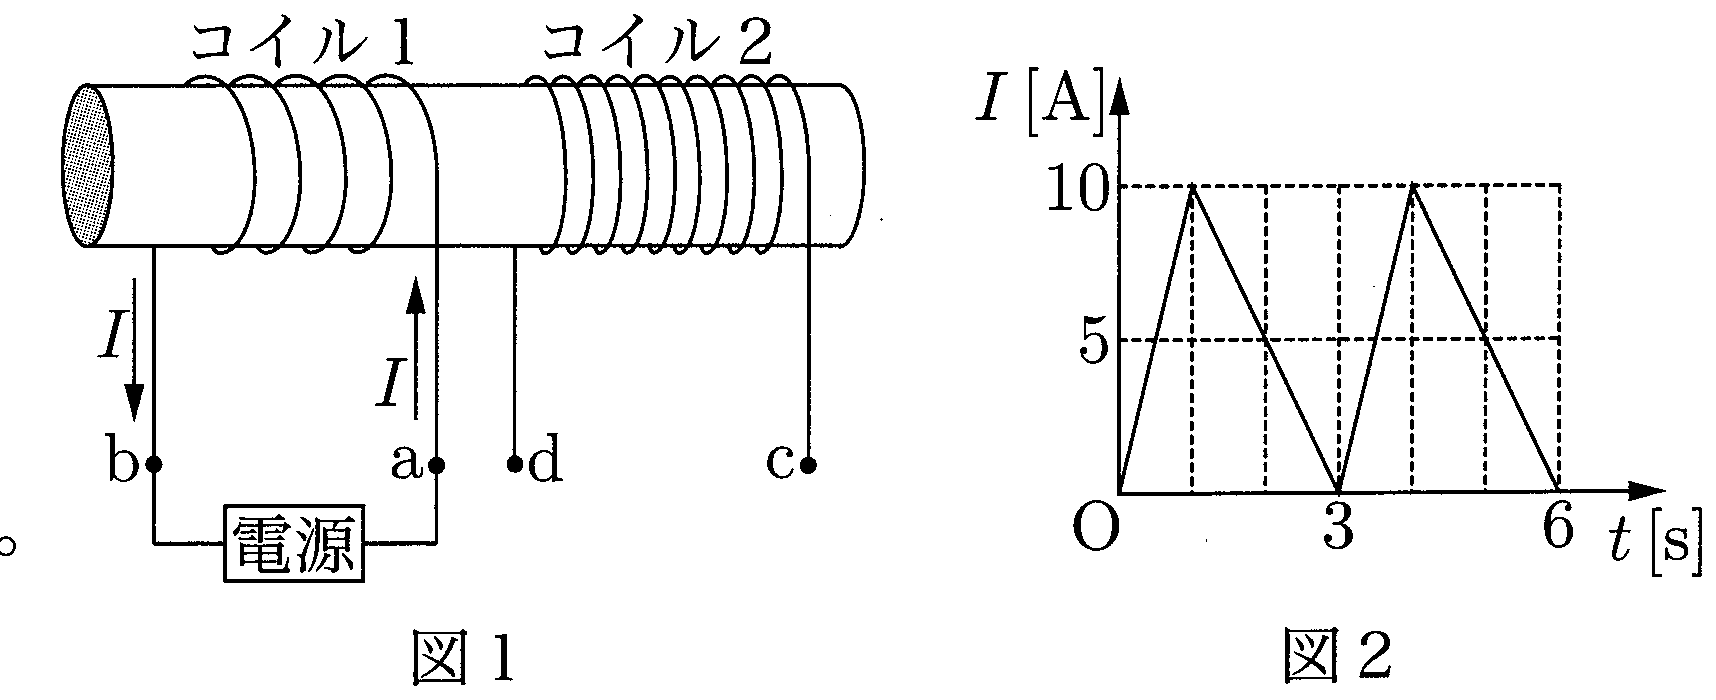
\includegraphics[keepaspectratio,width=100mm]{fig/n30_p105_zu.png}\end{center}

\Mon{変圧器}

\hspace{1zw}図1のような回路のコイル1に図2のような電流$I_1\U{A}$を流したとき，コイル2に生じる誘導起電力$V\U{V}$の時間変化を図に示せ．ただしコイル1，2間の相互インダクタンスを$0.50\U{H}$とし，$\mathrm{P}$に対して$\mathrm{Q}$の方が高電位になる場合を正として答えよ．
\begin{center}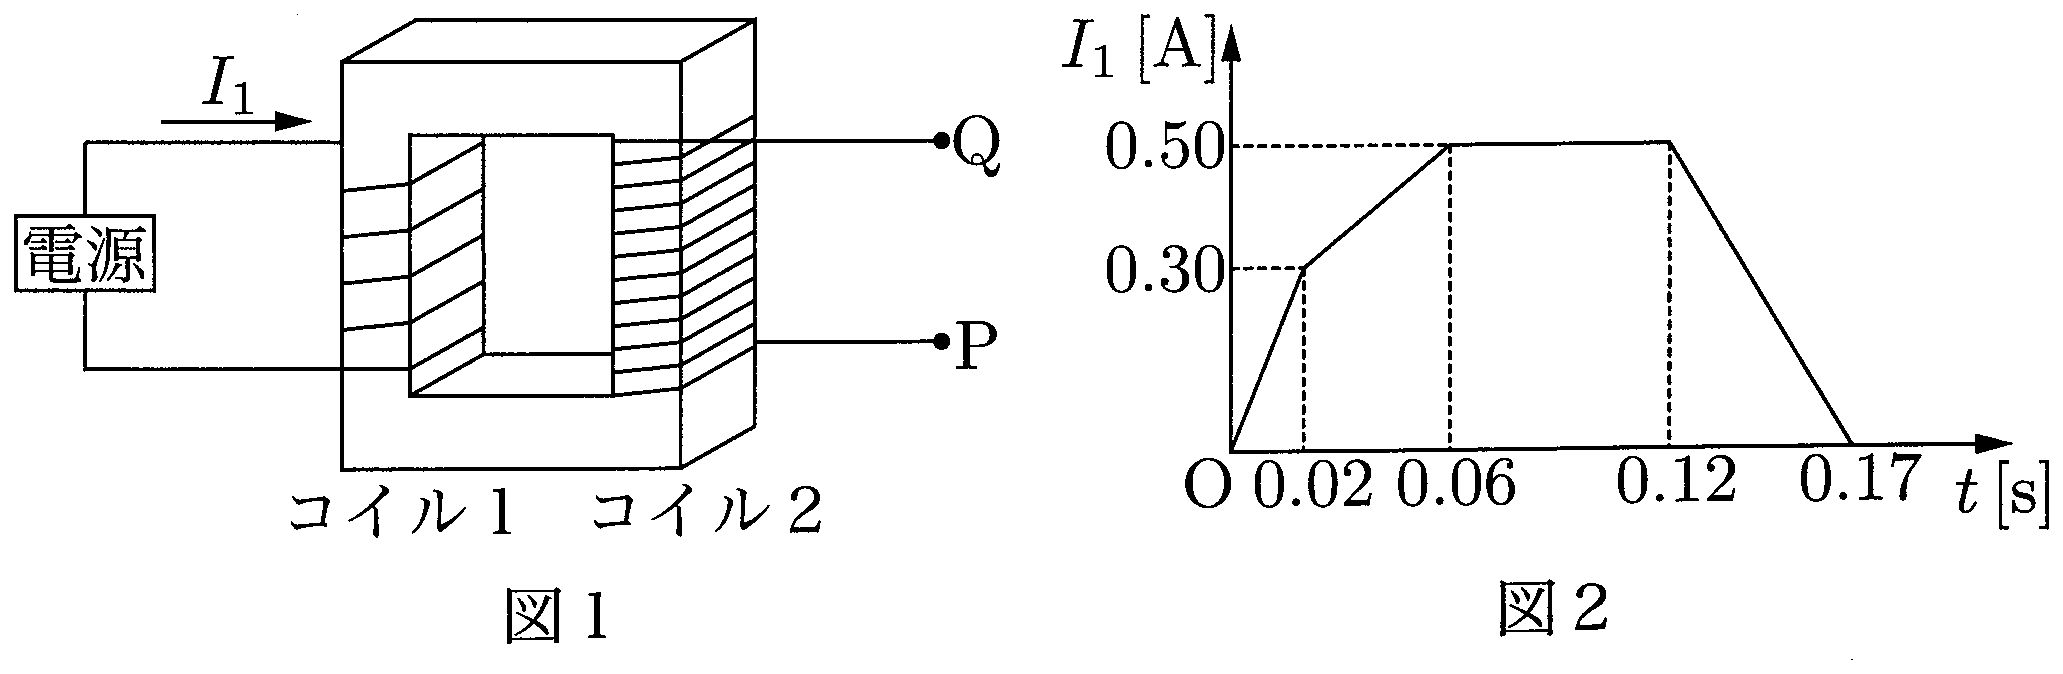
\includegraphics[keepaspectratio,width=110mm]{fig/n30_p106_zu.png}\end{center}

\Mon{相互インダクタンスの計算}

\begin{zuright}{56mm}
\hspace{1zw}右図のように断面積$S_1\U{m^2}$，総巻数$N_1$回，長さ$l_1\U{m}$のソレノイドコイル$\mathrm{P}$の内側に，断面積$S_2\U{m^2}$，総巻数$N_2$回，長さ$l_2\U{m}$のコイル$\mathrm{Q}$が中心軸を一致させて入れてある．$\mathrm{P}$の長さはその半径に比べて十分長く，また$l_1\gg l_2$であるとして以下の問いに答えよ．ただし，真空の透磁率を$\mu_0\U{N/A^2}$とする．
\begin{komon}
\ko{1} コイル$\mathrm{P}$の自己インダクタンス$L\U{H}$を求めよ．
\ko{2} コイル$\mathrm{P}$とコイル$\mathrm{Q}$の間の相互インダクタンス$M\U{H}$を求めよ．
\end{komon}
\zusep
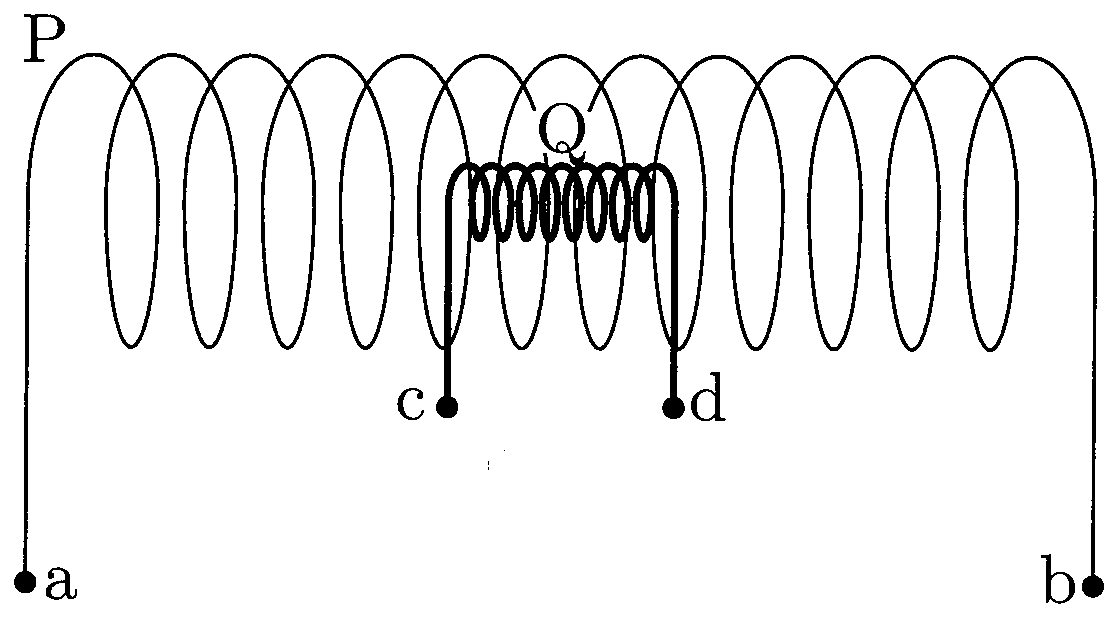
\includegraphics[keepaspectratio,width=54mm]{fig/n30_p107_zu.png}
\end{zuright}

% 原本の例題38（相互インダクタンス）を練習へ格下げした（`電磁気_例題配分.md`）．
\Mon{相互インダクタンス}

\begin{zuright}{46mm}
\hspace{1zw}図のように，半径$R\U{m}$，巻き数$N$の大きい円形コイル$\mathrm{A}$と，半径$r\U{m}$，巻き数$n$の小さい円形コイル$\mathrm{B}$とが，真空中で1つの平面上に同心に置かれている．コイル$\mathrm{A}$に電源をつなぎ，図の向きに電流$I\U{A}$を流した．真空の透磁率を$\mu_0\U{Wb^2/N\cdot m^2}$とし，$R\gg r$であるとする．
\begin{komon}
\ko{1} コイル$\mathrm{A}$によって円の中心位置につくられる磁場の大きさ$H\U{A/m}$を求めよ．
\ko{2} $R\gg r$であることを用いると，コイル$\mathrm{B}$を貫く磁力線はすべてコイルの面に対して垂直で，かつその磁束密度の大きさは中心位置における値に等しいと近似できる．このことを用いて，コイル$\mathrm{B}$を貫く磁束$\varPhi\U{Wb}$を求めよ．
\ko{3} 次に，この電流を微小時間$\varDelta t$の間に$\varDelta I$だけ増加させた．このとき，コイル$\mathrm{B}$に発生する誘導起電力の大きさ$V\U{V}$を求めよ．
\ko{4} コイル$\mathrm{A}$，$\mathrm{B}$間の相互インダクタンス$M\U{H}$を求めよ．
\end{komon}
\zusep
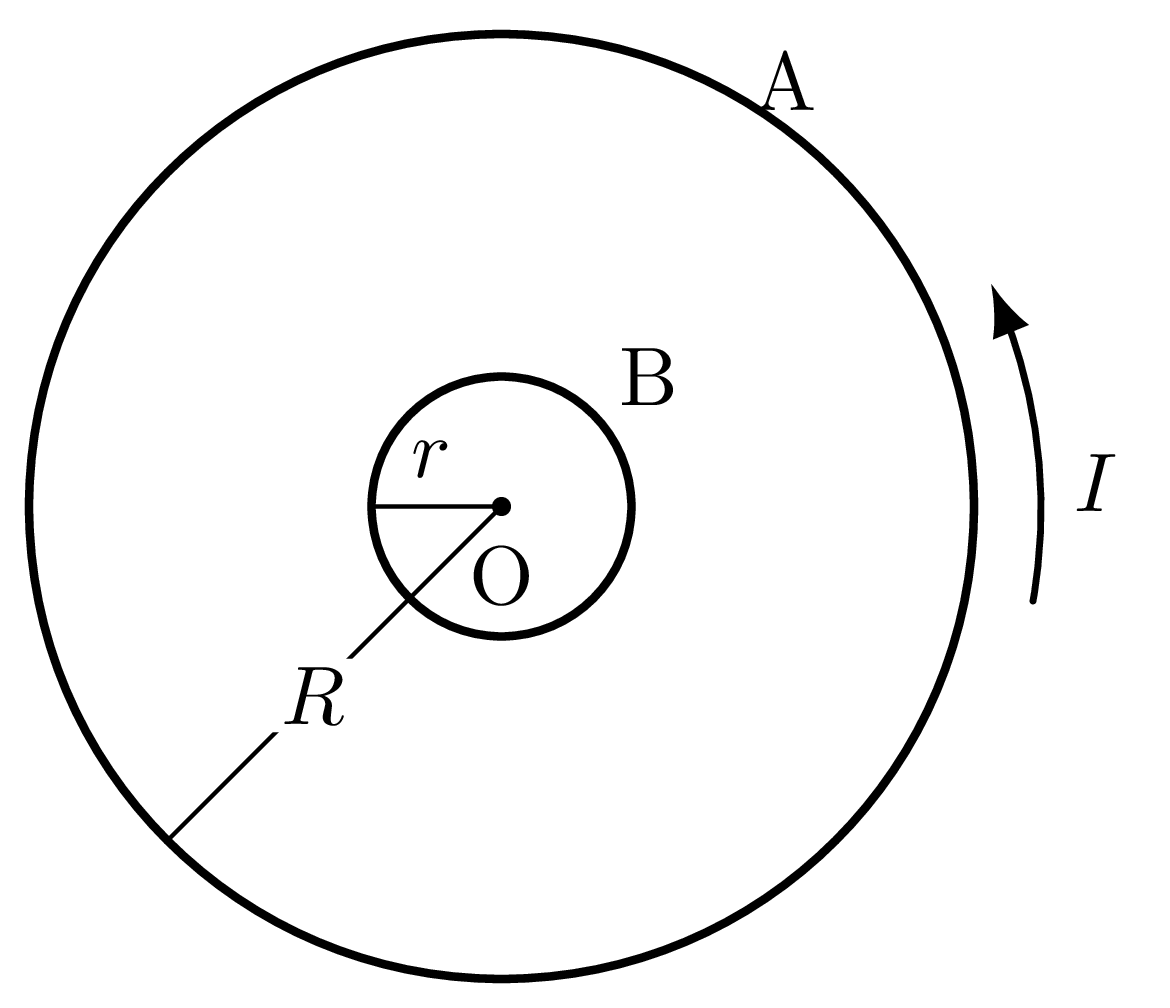
\includegraphics[keepaspectratio,width=44mm]{fig/n30_p108_zu.png}
\end{zuright}

\filbreak
\Rank{C問題}

\Mon{誘導電場}

\hspace{1zw}次の\framebox[4zw]{\rule{0pt}{1.1zw}1}から\framebox[4zw]{\rule{0pt}{1.1zw}4}に当てはまる適当な語句および数値を入れよ．
\begin{center}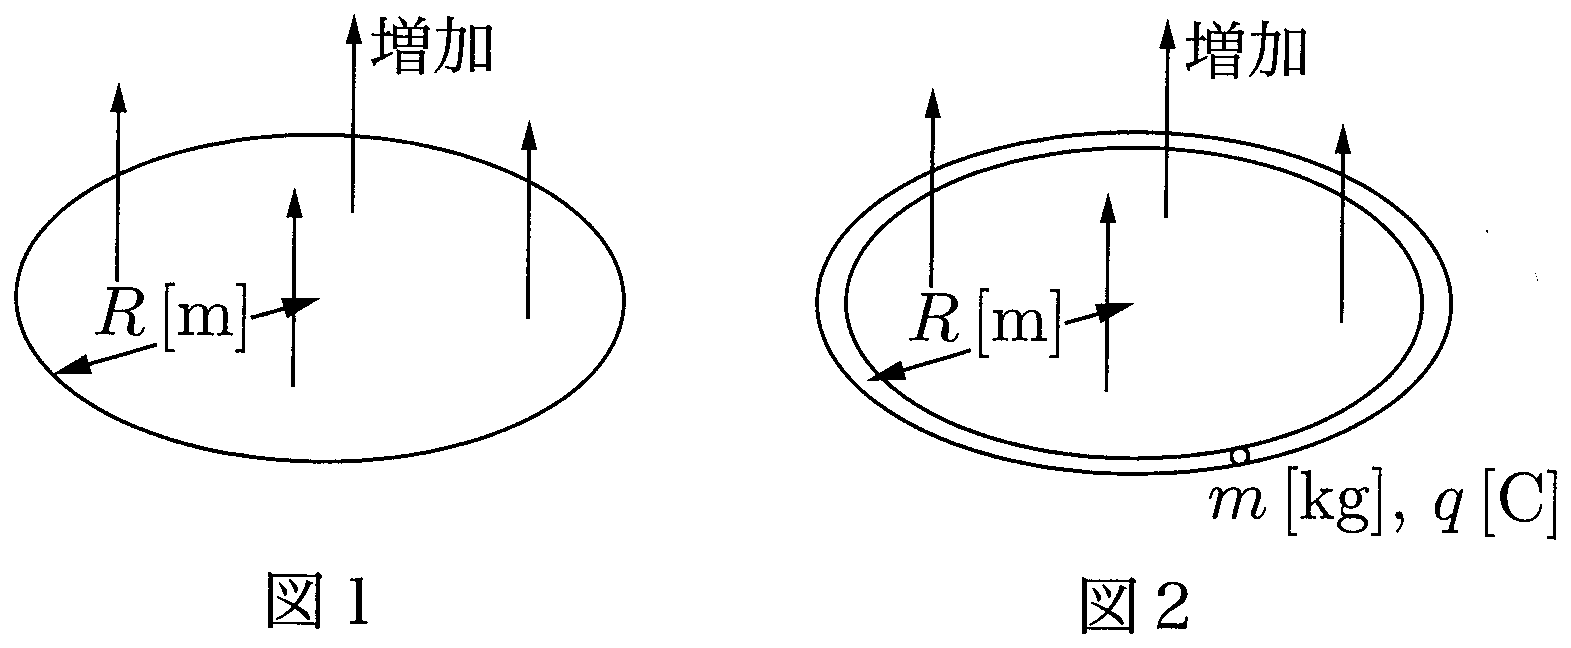
\includegraphics[keepaspectratio,width=88mm]{fig/n30_p109_zu.png}\end{center}
\hspace{1zw}図1のような半径$R\U{m}$の円形状導線に対して，上向きに一定の割合で増加する磁場をかけるとループに沿って誘導起電力が発生する．磁束密度の増加率を$\dfrac{dB}{dt}\U{Wb/m^2\cdot s}$とすると，このループひと回りに発生する誘導起電力の大きさ$V\U{V}$は\framebox[4zw]{\rule{0pt}{1.1zw}1}であるが，このような誘導起電力が生じるのは，磁束密度が変化するとき，そのまわりに誘導電場と呼ばれる電場が発生するからである．このループに沿った誘導電場の強さを$E\U{V/m}$とすると，$V=E\cdot 2\pi R$の関係より，$E=$\framebox[4zw]{\rule{0pt}{1.1zw}2}であることが分かる．また，誘導電場の向きは正電荷の受ける力の向きを考えると\framebox{\rule{0pt}{1.1zw}\,3：時計回り，反時計回り\,}であることが分かる．
\par
\hspace{1zw}このような誘導電場は，半径$R\U{m}$の位置に導線がなくても空間中に発生することができる．そのため，図2のように半径$R\U{m}$の中空のドーナツ状の円環を用意し，内部に質量$m\U{kg}$，電荷$q\U{C}$（$q>0$）の荷電粒子を置き，上向きに一定の割合$\dfrac{dB}{dt}\U{Wb/m^2\cdot s}$で増加する磁束密度をかけるとこの粒子は誘導電場により加速される．円環に沿ったこの粒子の加速度の大きさは\framebox[4zw]{\rule{0pt}{1.1zw}4}となる．

\Mon{相互誘導起電力}

\begin{zuright}{58mm}
\hspace{1zw}次の\framebox[4zw]{\rule{0pt}{1.1zw}1}から\framebox[4zw]{\rule{0pt}{1.1zw}4}に当てはまる適当な語句および数値を入れよ．
\par
\hspace{1zw}右図のように鉄棒に銅線を巻いて作ったコイル$\mathrm{AB}$，電池$\mathrm{E}$，抵抗$\mathrm{R}$からなる回路のそばに，銅環$\mathrm{L}$を中心軸が鉄心の中心軸に一致するように糸でつるして置く．
\zusep
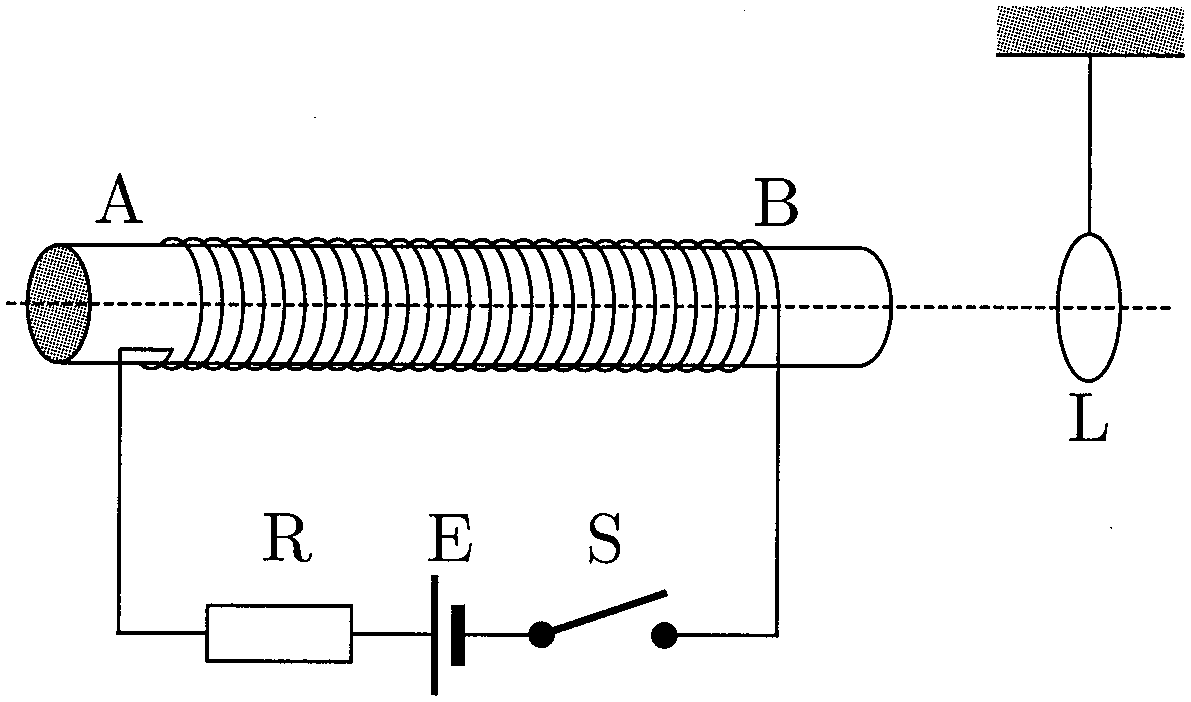
\includegraphics[keepaspectratio,width=56mm]{fig/n30_p110_zu.png}
\end{zuright}
今，スイッチ$\mathrm{S}$を閉じるとき，コイルに流れる電流は次第に増加するので，$\mathrm{L}$には$\mathrm{AB}$側から見て\framebox{\rule{0pt}{1.1zw}\,1：時計回り，反時計回り\,}に誘導電流が流れる．この電流は$\mathrm{AB}$に流れる電流と\framebox{\rule{0pt}{1.1zw}\,2：同じ，逆\,}向きに流れているので，$\mathrm{L}$は$\mathrm{AB}$に\framebox{\rule{0pt}{1.1zw}\,3：反発さ，引き付けら\,}れる．続いて$\mathrm{S}$を開くと，$\mathrm{L}$は$\mathrm{AB}$に\framebox{\rule{0pt}{1.1zw}\,4：反発さ，引き付けら\,}れる．

\newpage

%%%%%%%%%%%%%%%%%%%%  解答  %%%%%%%%%%%%%%%%%%%%
\KaiTitle{第30回　電磁誘導・自己誘導・相互誘導}
\setlength{\columnseprule}{0.4pt}
\begin{multicols}{2}
\raggedcolumns

\Rank{A問題}
\MonN{99}{基本公式の確認}\par\nopagebreak
\begin{sisin}
誘導起電力の向きは，\MARU{1}ループを貫く磁束がどう変化するのかを押さえる，\MARU{2}その磁束変化を緩和するためにはどちら向きの磁場が発生すればよいのかを考える，\MARU{3}その磁場をつくるためにはどちら向きに電流が流れればよいのかを考える，\MARU{4}その電流を流すためにはどちら向きに起電力が発生すればよいのかを考える，という手順を踏んで考えればよい．

誘導起電力はループを貫く磁場が{\gtfamily 変化する}ときに初めて発生するものであることに注意せよ．磁場が存在していても変化しなければ誘導起電力は発生しない．また，ループが$N$回巻きの場合，誘導起電力は$-N\dfrac{d\varPhi}{dt}$となる．

(4)(5)の相互誘導起電力については二つのコイルの配置，巻き方の向きなどを考慮する必要があるため一概にどちら向きとは決められない．必ず，\MARU{1}一次コイルがつくる磁場の向き，\MARU{2}その磁場と同じ向きの磁場を生じる二次コイルの電流の向き，\MARU{3}その向きの電流を流そうとする起電力の向きを正，という手順で考えること．
\end{sisin}
\KaiHead
\begin{komon}
\ko{1} 図1の場合，次図のように磁場がつくられている．
       \begin{center}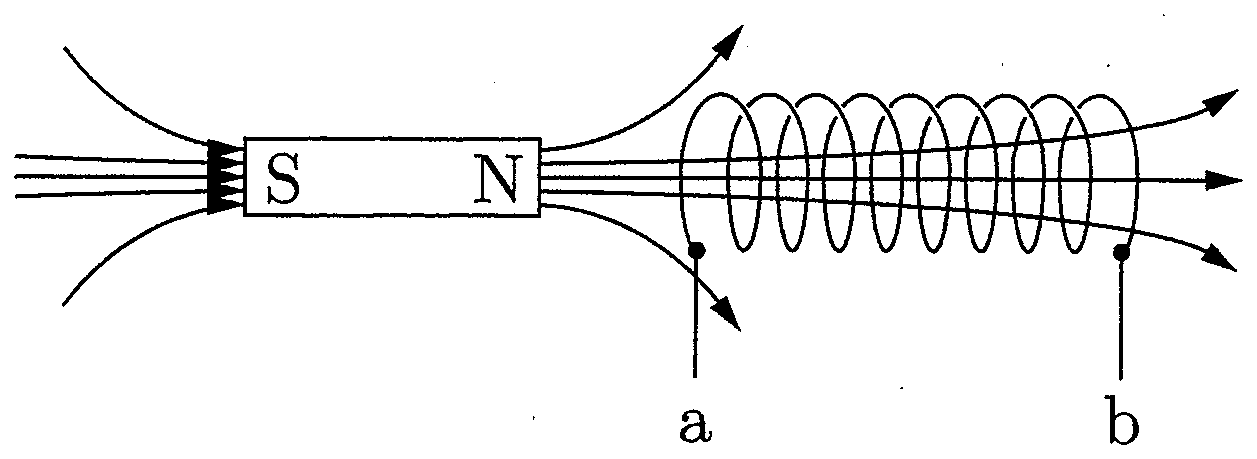
\includegraphics[keepaspectratio,width=56mm]{fig/n30_a99_zu1.png}\end{center}
       \MARU{1}\ N極がつくる磁場は磁石に近いほど強いので，磁石をコイルに近づけると，コイルを右向きに貫く磁場が増加する．この磁束変化を緩和するには左向きの磁場をつくればよいので，コイルを$\mathrm{b}\to\mathrm{a}$の向きに誘導電流が流れるように誘導起電力が発生する（しかし，誘導電流は流れない）．よって，{\gtfamily $\mathrm{a}$}の方が高電位となる．\Ans

       \MARU{2}\ コイルを下方向へずらすとコイルを右向きに貫く磁束は減少する．この磁束変化を緩和するには右向きの磁場をつくればよいので，$\mathrm{a}\to\mathrm{b}$の向きに誘導電流が流れるように誘導起電力が発生する．よって，{\gtfamily $\mathrm{b}$}の方が高電位となる．\Ans

       また図2の場合，もし左側のコイルに電流が流れた場合には次図のような磁場がつくられる．
       \begin{center}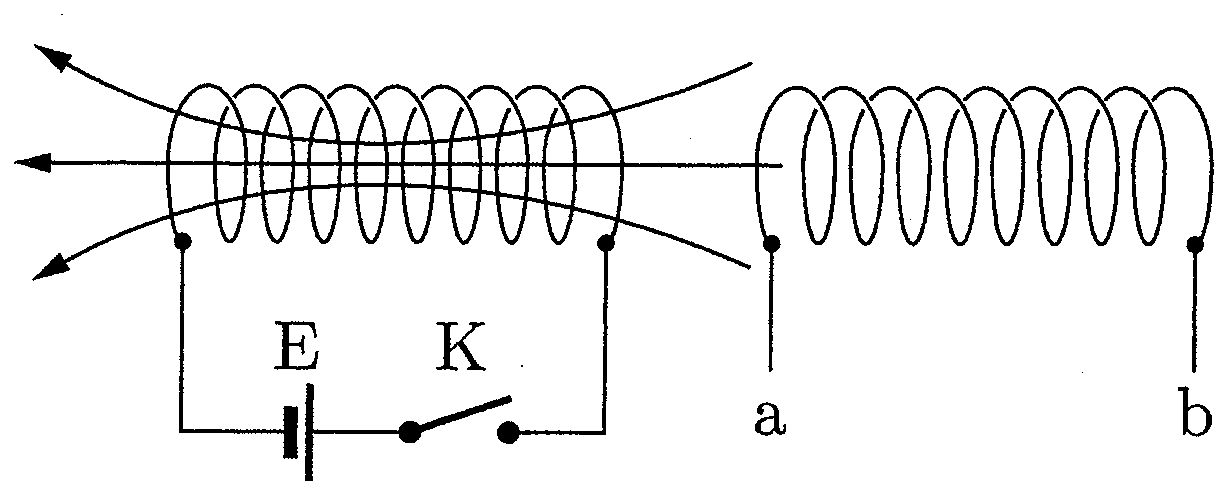
\includegraphics[keepaspectratio,width=56mm]{fig/n30_a99_zu2.png}\end{center}
       \MARU{3}\ スイッチを入れると前図のような磁場が発生するので，右のコイルを左向きに貫く磁場が増加する．この磁束変化を緩和するには右向きの磁場が発生すればよいので，$\mathrm{a}\to\mathrm{b}$向きに誘導電流が流れるように誘導起電力が発生する．よって，{\gtfamily $\mathrm{b}$}の方が高電位となる．\Ans

       \MARU{4}\ スイッチを入れて十分時間が経過すると，左側のコイルを流れる電流は一定値になるため，左のコイルがつくる磁場は一定となる．よって，右側のコイルを貫く磁場は変化しないので，誘導起電力は発生しない．以上より，{\gtfamily $\mathrm{a}$，$\mathrm{b}$の電位は等しい}．\Ans
\ko{2} \[\begin{aligned}
         V&=\left|-N\frac{d\varPhi}{dt}\right|=\left|-N\frac{dB}{dt}S\right|\\
         &=500\cdot\frac{4.0\times 10^{-2}}{2.0\times 10^{-2}}\cdot 3.0\times 10^{-4}\\
         &=3.0\times 10^{-1}\U{V}\Ans
       \end{aligned}\]
\ko{3} \[\left|-L\frac{dI}{dt}\right|=30\cdot\frac{0.10}{2.0}=1.5\U{V}\Ans\]
\ko{4} $\mathrm{S}$を閉じるとコイル$\mathrm{A}$には電流が流れ，そのとき生じる磁場の向きは，右ねじの法則より上向きである．コイル$\mathrm{B}$が上向きの磁場を生じるためには$\mathrm{a}$の向きに電流が流れればよく，この向きが正である．相互誘導起電力は$-M\dfrac{dI_1}{dt}$で，$\mathrm{S}$を閉じると$\dfrac{dI_1}{dt}>0$なので負になる．よって負の向き，すなわち{\gtfamily $\mathrm{b}$}の向きに電流が流れる．\Ans
\ko{5} \[\left|-M\frac{dI_1}{dt}\right|=4.0\cdot\frac{2.0}{0.50}=16\U{V}\Ans\]
\end{komon}

\Rank{B問題}
\MonN{100}{回路に生じる誘導起電力}\par\nopagebreak
\begin{sisin}
本問では磁束が増減するので誘導起電力の大きさだけで考えることはできない．ファラデーの電磁誘導の法則$V=-\dfrac{d\varPhi}{dt}$の式に従って考えていくことになる．

$V=-\dfrac{d\varPhi}{dt}$の示す正の向きは，元ある磁束の向きと同じ向きの磁場を発生させるような電流の向きを正とし，そのような電流を流すような起電力の向きを正としている．この向きと問題で設定されている正の向きが一致しているかどうかチェックすること．
\end{sisin}
\KaiHead
元ある磁束の向き（上向き）と同じ向きの磁場を発生させる誘導電流の向きは，反時計回りの向きである．この向きに電流を流す起電力の向きが正であるから，ファラデーの電磁誘導の法則より，$V=-\dfrac{d\varPhi}{dt}$である．また，与えられたグラフより
\[V=-\frac{d\varPhi}{dt}=\left\{\begin{aligned}
  &-10\quad(0<t<0.01)\\
  &-5\quad(0.01<t<0.02)\\
  &\ 0\quad(0.02<t<0.03)\\
  &15\quad(0.03<t<0.04)
\end{aligned}\right.\]
である．これより，グラフをプロットすると次図のようになる．\Ans
\begin{center}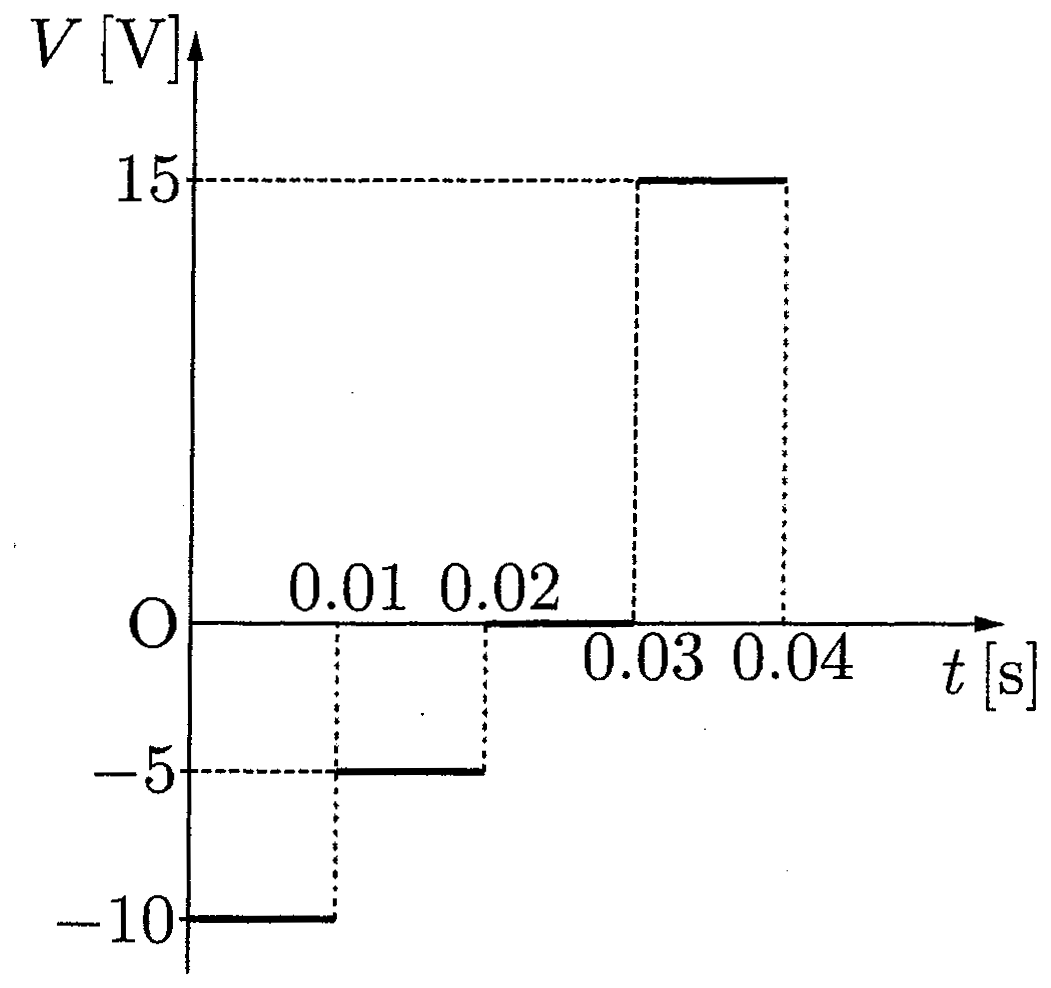
\includegraphics[keepaspectratio,width=46mm]{fig/n30_a100_zu.png}\end{center}

\MonN{101}{矩形コイルの電磁誘導}\par\nopagebreak
\begin{sisin}
導体棒上に発生する誘導起電力の考え方には2通りある（30.2）．両方とも覚えておき，自分なりに使いやすい方を利用せよ．
\MARU{1}\ 導体棒が微小時間$dt$の間に掃く面積$dS$を計算し，磁束$=$磁束密度$\times$面積の関係からこの間に掃く磁束$d\varPhi=B\cdot dS$を求め，これから発生する誘導起電力を求める．
\MARU{2}\ 導体棒中の自由電子が導体棒とともに動くと考え，自由電子に作用するローレンツ力から発生する誘導起電力の大きさ$vBl$を求める．
いずれの場合についても，最終的には導体棒を誘導起電力分の起電力を持つ電池だと考えてしまうとキルヒホッフの第二法則を利用することができる．
\end{sisin}
\KaiHead
\begin{komon}
\ko{1} $\mathrm{PX}=x$とおき，回路を上向きに貫く磁束を$\varPhi$とおく．$\varPhi=Blx$，$\dfrac{dx}{dt}=-v$であるから，ファラデーの電磁誘導の法則より，求める誘導起電力の大きさは，
       \[\left|-\frac{d\varPhi}{dt}\right|=|-(-Blv)|=Blv\U{V}\Ans\]
       また，回路を上向きに貫く磁束が減少するから，$\mathrm{P}\to\mathrm{Q}$の向きに誘導電流が流れる．よって，誘導起電力の向きは，{\gtfamily $\mathrm{P}\to\mathrm{Q}$向き}\Ans
       \begin{bekkai}
       導体棒内の自由電子が導体棒と同じ速さで磁場中を運動していると考えると，自由電子に作用するローレンツ力の大きさは$f=evB$．この力と同じ大きさのクーロン力を及ぼす電場の大きさを$E$とすると，$eE=f$より$E=vB$．この電場が導体棒中に一様にできているといえるので，導体棒の両端の電位差は$El=vBl$．これが求める起電力の大きさに他ならない．また，電子が受けるローレンツ力の向きはフレミングの左手の法則より$\mathrm{Q}\to\mathrm{P}$向きなので，電子が$\mathrm{P}$側に集まり，$\mathrm{Q}$の方が高電位になっている．
       \end{bekkai}
       \begin{center}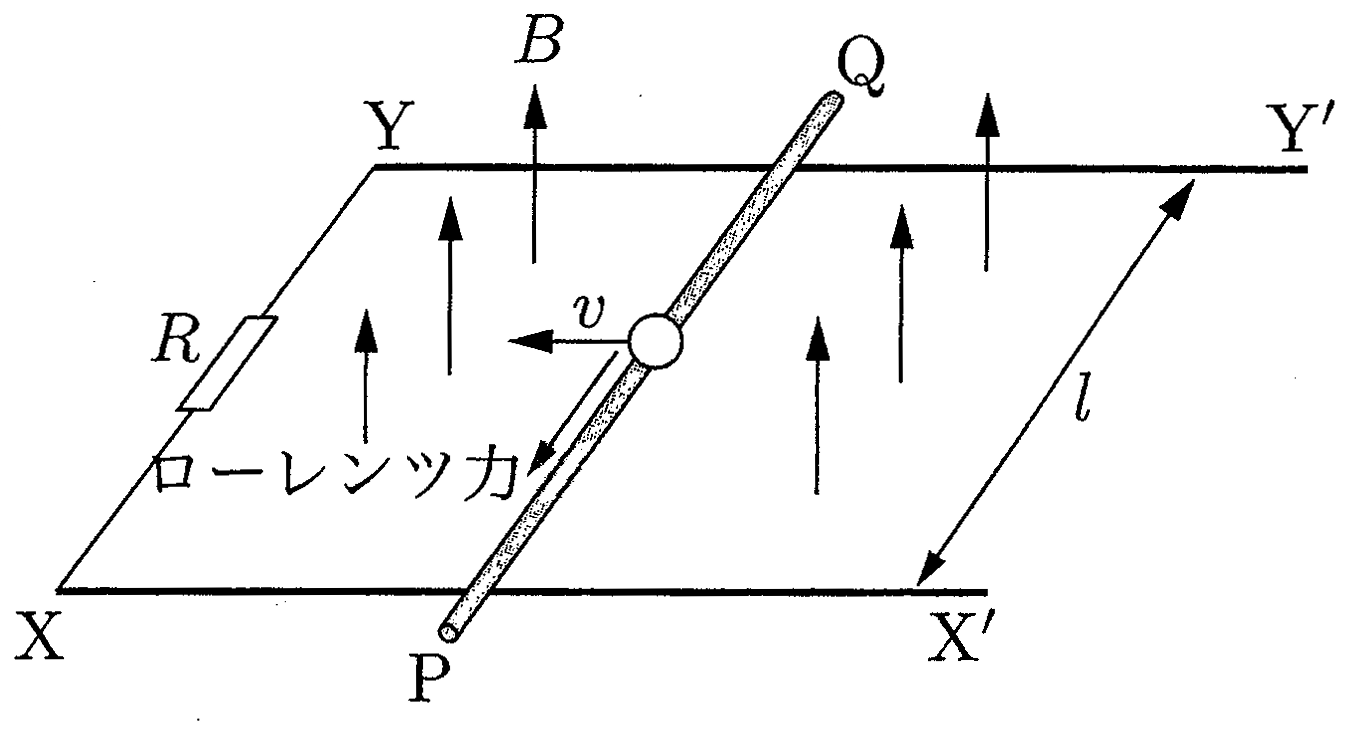
\includegraphics[keepaspectratio,width=56mm]{fig/n30_a101_zu1.png}\end{center}
\ko{2} (1)より導体棒$\mathrm{PQ}$には大きさ$vBl$の誘導起電力が発生しているので，これを電池とみなして回路を描くと次図のようになる．
       \begin{center}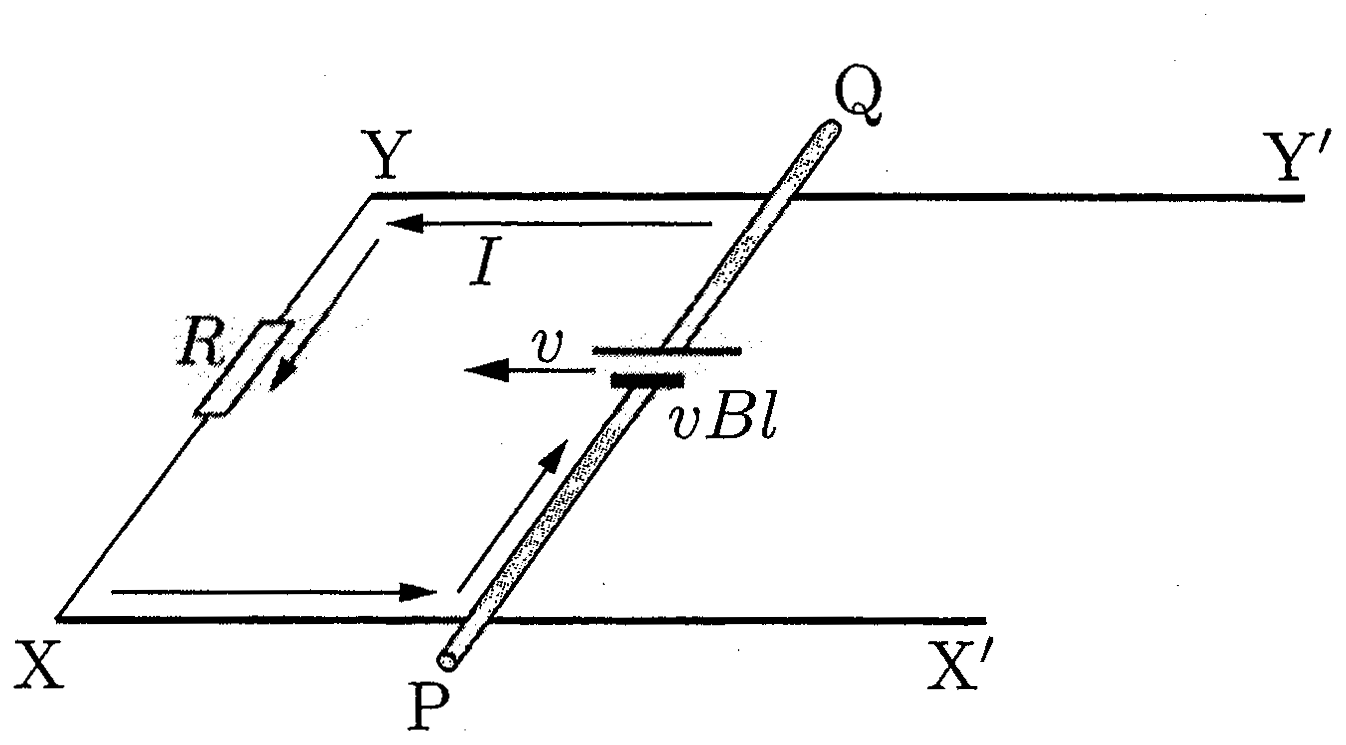
\includegraphics[keepaspectratio,width=56mm]{fig/n30_a101_zu2.png}\end{center}
       この回路に生じる誘導電流の大きさを$I$とすれば，キルヒホッフの第二法則より，$vBl=RI$が成立するので，
       \[I=\frac{vBl}{R}\U{A}\Ans\]
       また，誘導電流の流れる向きは，$\mathrm{P}\to\mathrm{Q}\to\mathrm{Y}\to\mathrm{X}$\Ans
\ko{3} $\mathrm{P}\to\mathrm{Q}$向きに流れるこの電流はフレミングの左手の法則より$\mathrm{X}\to\mathrm{X}^\prime$の向きに大きさ$IBl$の電磁力を受ける．導体棒$\mathrm{PQ}$が一定の速さで動くためには力がつり合っていなければならないので，電磁力と等大逆向きの外力が作用していなければならない．
       \begin{center}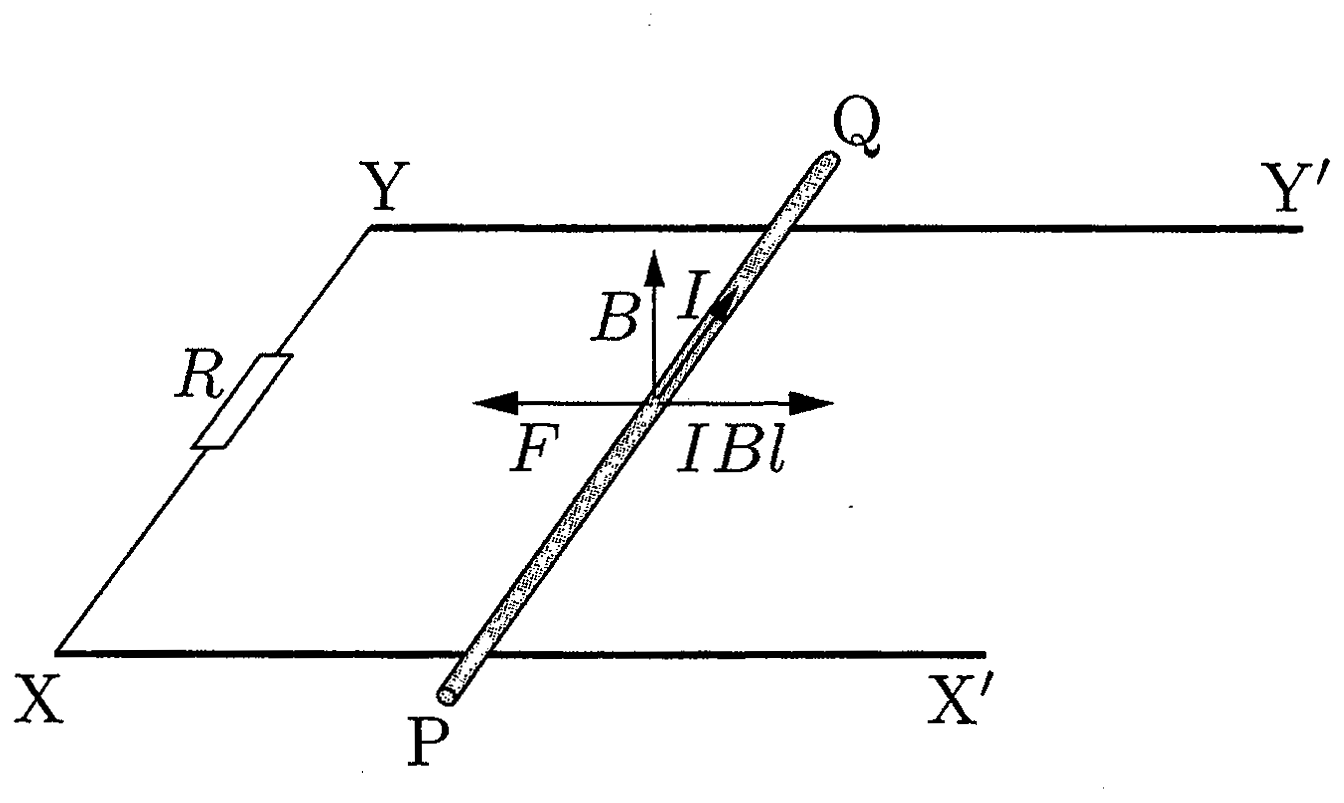
\includegraphics[keepaspectratio,width=56mm]{fig/n30_a101_zu3.png}\end{center}
       以上より，加えている外力の大きさおよび向きは，
       \[\left\{\begin{aligned}
         &\text{大きさ：}\ IBl=\frac{vB^2l^2}{R}\U{N}\\
         &\text{向き：}\ \mathrm{X}^\prime\to\mathrm{X}
       \end{aligned}\right.\Ans\]
\end{komon}

\MonN{102}{ローレンツ力と電磁誘導}\par\nopagebreak
\begin{sisin}
磁場を横切って動く導体棒に誘導起電力が発生するのは，本問にあるように，導体棒と共に動く電子がローレンツ力を受けるため，その効果を起電力が生じた効果に置き換えることができるからである（30.2）．誘導に沿って答えていけば簡単な問題であろう．
\end{sisin}
\KaiHead
\begin{komon}
\item[{\makebox[1.9zw][r]{(1)(2)}}] 次図のように電子の動きを考えれば，電子が負電荷であることに注意してフレミングの左手の法則を利用して，
       \[\left\{\begin{aligned}
         &\text{向き：}\ \mathrm{Q}\to\mathrm{P}\quad\cdots\text{(1)の(答)}\\
         &\text{大きさ：}\ evB\U{N}\quad\cdots\text{(2)の(答)}
       \end{aligned}\right.\]
       \begin{center}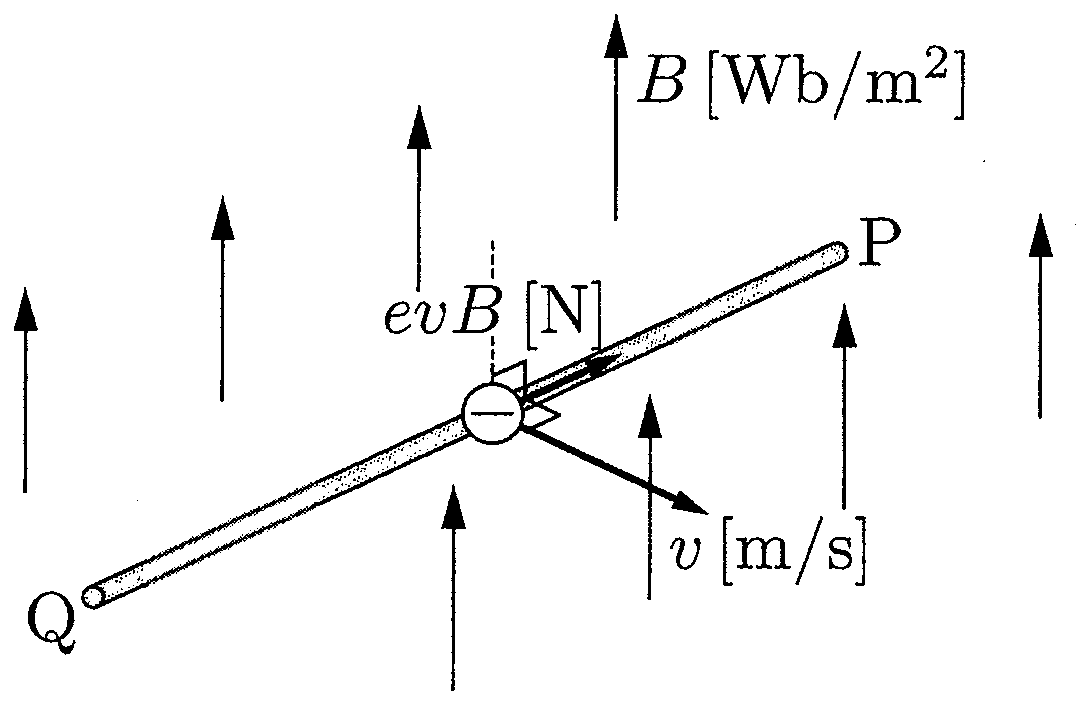
\includegraphics[keepaspectratio,width=48mm]{fig/n30_a102_zu.png}\end{center}
\item[{\makebox[1.9zw][r]{(3)(4)}}] 導体が運動することにより，電子が$\mathrm{Q}\to\mathrm{P}$の向きに大きさ$evB$のローレンツ力を受けることになるが，これは$\mathrm{P}\to\mathrm{Q}$の向きに大きさ$E=vB$の電場が存在するときに受ける力と全く同一である（電子は負電荷であるから電場と逆向きに力を受けることに注意）．つまり，導体棒が動いたという効果は，電子にとっては
       \[\left\{\begin{aligned}
         &\text{向き：}\ \mathrm{P}\to\mathrm{Q}\ \text{の向き}\quad\cdots\text{(3)の(答)}\\
         &\text{大きさ：}\ E=vB\U{V/m}\quad\cdots\text{(4)の(答)}
       \end{aligned}\right.\]
       の電場が生じたのと同じ効果を持っている．
\ko{5} 以上より，
       \[V=E\cdot l=vBl\U{V}\Ans\]
\end{komon}
\begin{chuu}
問題文から『ローレンツ力を受けることで導体棒$\mathrm{PQ}$内に電場が生じる』と読み取りがちであるが，実際に導体棒$\mathrm{PQ}$内に電場が生じているわけではないことに注意せよ（つまり電子はクーロン力を受けているのではない）．ここでは，ローレンツ力による効果を電場による効果に置き換えるという議論をしているだけである．

また，仮想電場の向きが$\mathrm{P}\to\mathrm{Q}$の向きであり，電場は電位の高い方から低い方に向かうから$\mathrm{P}$が電池の高電位側である，と考えるのは誤りである．ここで考えた電場はあくまで仮想的なものであるから，必ずしも通常の電場と電位の向きの関係を満たしてはいない．

なお，誘導起電力の発生のメカニズムには2通りあり，本問のようなタイプとC問題［109］のようにして発生するタイプ（誘導電場）の2通りがある（30.2）．
% 原本は「C問題［20］」（旧回の番号）．
\end{chuu}

\MonN[\Sitei]{103}{終端速度}\par\nopagebreak
\begin{sisin}
回路に電池をつなぐとそれにより電流が流れ，金属棒が電磁力を受けることにより加速していくが，ある程度まで加速すると棒の速度はそれ以上増加しなくなり，これを終端速度と呼ぶ．運動方程式を速度$v$に関する微分方程式にまとめるのが基本方針であるが，その方程式をどう解釈すればよいのかまで含めてきっちり押さえておくこと（30.3）．
\end{sisin}
\KaiHead
\begin{komon}
\ko{1} 導体棒が右向きの速度$v$で動いている場合，この導体棒には$\mathrm{P}\to\mathrm{Q}$の向きに大きさ$vBl$の誘導起電力が発生する（導体棒が右向きに動く場合には，ループ$\mathrm{XPQX}^\prime$を貫く下向きの磁束が増加するので，レンツの法則より誘導電流が$\mathrm{P}\to\mathrm{Q}$の向きに流れるような誘導起電力が生じる）．よって，キルヒホッフの第二法則より，$E=vBl+RI$と立式でき，これを解くと，
       \[I=\frac{E-vBl}{R}\U{A}\Ans\]
       \begin{center}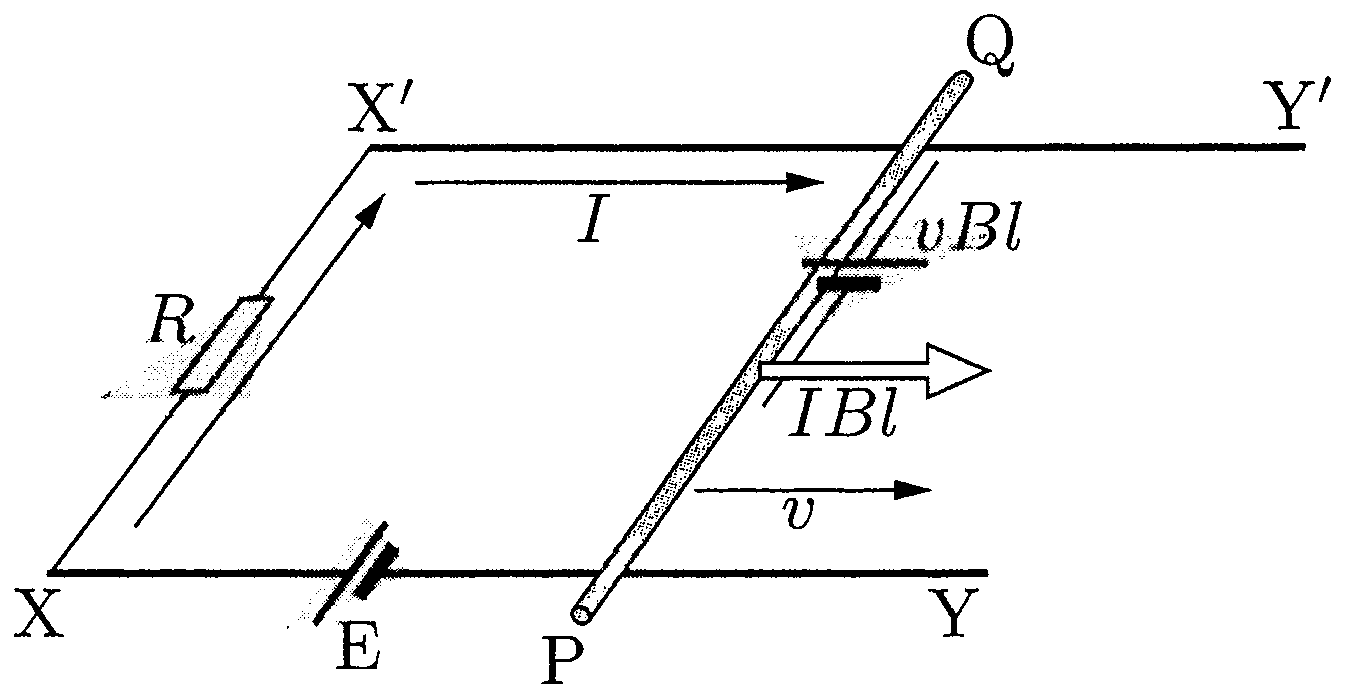
\includegraphics[keepaspectratio,width=56mm]{fig/n30_a103_zu.png}\end{center}
       またこのとき，導体棒は電流$I$により大きさ$IBl$の電磁力を受ける．フレミングの左手の法則より電磁力の向きは右向きであるから，導体棒の運動方程式は，$ma=IBl$となる．先に求めた$I$を代入すると，
       \[ma=\Bigl(\frac{E-vBl}{R}\Bigr)Bl\Ans\]
\ko{2} 加速度$a$と速度$v$の間には$a=\dfrac{dv}{dt}$の関係が成立するので，(1)の運動方程式は
       \[\frac{dv}{dt}=\frac{EBl}{mR}-\frac{B^2l^2}{mR}v\]
       とまとめられる．始めは$v=0$であり，$\dfrac{dv}{dt}=\dfrac{EBl}{mR}>0$であるから速度$v$は増加していくが，$v$が増加していくと$\dfrac{dv}{dt}$は次第に減少していくので，速度の増加率はだんだん小さくなっていく．そして$\dfrac{dv}{dt}=0$となると速度はそれ以上増加しなくなるので，物体の速度は下のグラフのように変化することが分かる．
       \begin{center}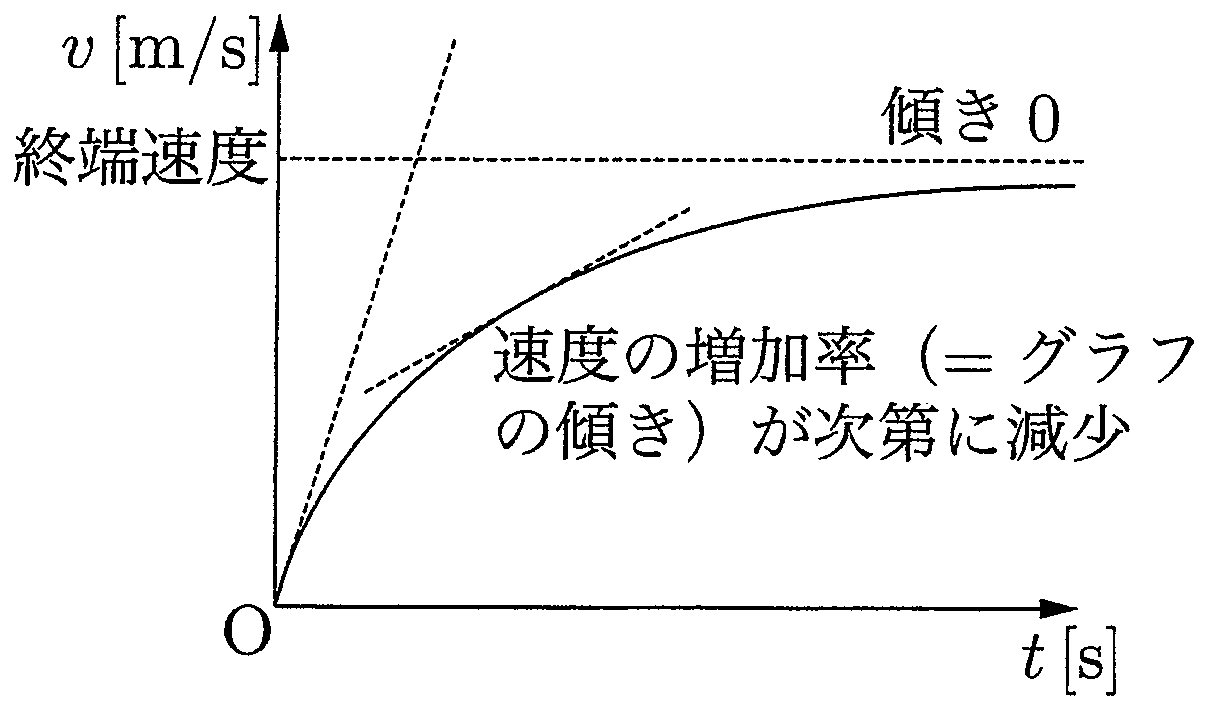
\includegraphics[keepaspectratio,width=56mm]{fig/n30_a103_graph.png}\end{center}
       よって，終端速度は$\dfrac{dv}{dt}=0$となったときの速度であるから，これを解いて，
       \[v=\frac{E}{Bl}\U{m/s}\Ans\]
       またこのときに流れる電流は，(1)の答えにこの値を代入して$I=0$であるから，抵抗での消費電力は
       \[P=RI^2=0\U{W}\Ans\]
\end{komon}
\begin{bsHosoku}{参考}
最後の問題は以下のように考えてもよい．一定の速度（終端速度）に達したときには導体棒には力が作用していない（力が作用していると速度が変化してしまう）ので，流れている電流は$0$と分かる．よって，消費電力は$0$になる．

(1)の運動方程式を整理した式は微分方程式であり，これを解くと（高校範囲外），$\dfrac{dv}{v-\frac{E}{Bl}}=-\dfrac{B^2l^2}{mR}dt$と変数を分けて積分し，$t=0$で$v=0$を用いて
\[v(t)=\frac{E}{Bl}\Bigl(1-e^{-\frac{B^2l^2}{mR}t}\Bigr)\]
となり，$t\to\infty$で$v\to\dfrac{E}{Bl}$となる．

また，エネルギー保存則として，電池が電流を流すことにより行う仕事が，抵抗でのジュール熱と導体棒の運動エネルギーの増加に転化している．実際，
\[RI^2+mv\frac{dv}{dt}=RI^2+IBl\cdot v=I(RI+vBl)=IE\]
であり，$IE$は電池が単位時間あたりにする仕事である．
\end{bsHosoku}

\MonN[\Sitei]{104}{回路の運動}\par\nopagebreak
\begin{sisin}
本問のように，長方形ループが磁場中に入っていくタイプの問題は入試でもよく見受けられるが，攻め方としては，
\MARU{1}\ 時刻$t$においてループを貫く全磁束$\varPhi$を場合分けして求めておき，これから発生する誘導起電力$-\dfrac{d\varPhi}{dt}$をファラデーの電磁誘導の法則より求める
\MARU{2}\ 導体棒中の電子が受けるローレンツ力から導体棒上に誘導起電力$vBl$の電池を置いて考える
のどちらでも正しく答えを求めることができるが，計算の容易さという観点からは後者の方がラクである．前者による解き方は別解として示す．
% 原本は「B問題［16］と同様に」（旧回の番号）．
\end{sisin}
\KaiHead
辺$\mathrm{AD}$，$\mathrm{BC}$の二つは磁場中に入っても磁場を垂直に掃かないので，誘導起電力を生じない．磁場を垂直に掃く辺$\mathrm{AB}$，$\mathrm{DC}$の二つに誘導起電力が発生する．辺$\mathrm{AB}$，$\mathrm{DC}$中の電子が受けるローレンツ力の向きはフレミングの左手の法則より$\mathrm{A}\to\mathrm{B}$，$\mathrm{D}\to\mathrm{C}$であり，辺の両端の電位差は$vBa$となる．電子の移動の向きから高電位となるのは$\mathrm{A}$，$\mathrm{D}$である．
\begin{center}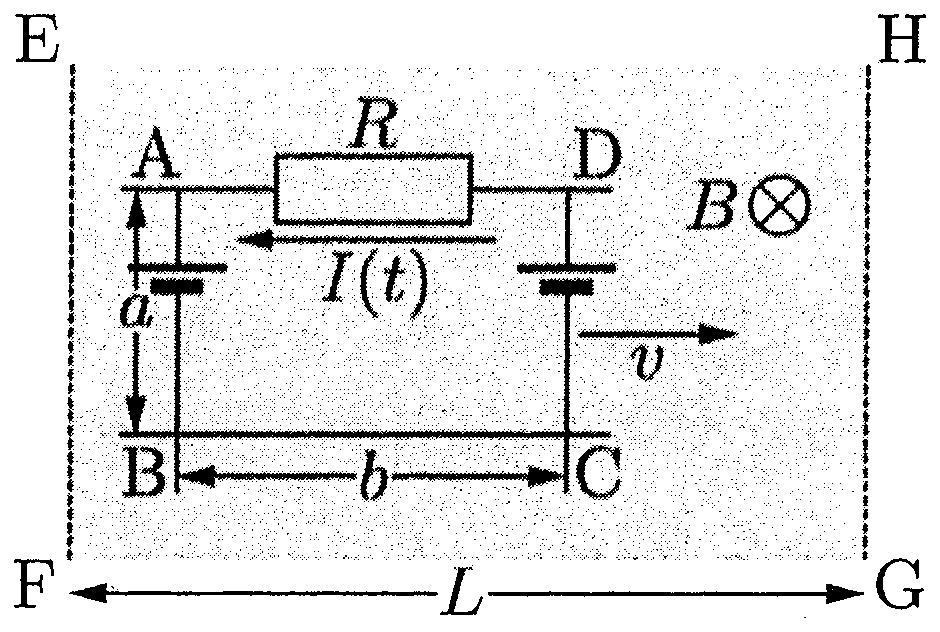
\includegraphics[keepaspectratio,width=50mm]{fig/n30_a104_zu.png}\end{center}
長方形回路が磁場を横切っていく途中過程は以下の四つに分けられる．
\begin{komon}
\item[{\makebox[1.9zw][r]{\MARU{1}}}] $0<t<\dfrac{b}{v}$のとき：辺$\mathrm{DC}$上のみに$vBa$の誘導起電力が発生するので，キルヒホッフの第二法則より$vBa=RI(t)$となり，
       \[I(t)=\frac{vBa}{R}\U{A}\Ans\]
\item[{\makebox[1.9zw][r]{\MARU{2}}}] $\dfrac{b}{v}<t<\dfrac{L}{v}$のとき：辺$\mathrm{AB}$，$\mathrm{DC}$の両方の上に$vBa$の誘導起電力が発生し，$vBa-vBa=RI(t)$となる．よって，
       \[I(t)=0\U{A}\Ans\]
\item[{\makebox[1.9zw][r]{\MARU{3}}}] $\dfrac{L}{v}<t<\dfrac{L+b}{v}$のとき：辺$\mathrm{AB}$上のみに$vBa$の誘導起電力が発生するので，$-vBa=RI(t)$となり，
       \[I(t)=-\frac{vBa}{R}\U{A}\Ans\]
\item[{\makebox[1.9zw][r]{\MARU{4}}}] $t>\dfrac{L+b}{v}$のとき：長方形コイルは磁場の右側へすべて出てしまっているので誘導起電力は発生しない．よって，
       \[I(t)=0\U{A}\Ans\]
\end{komon}
\begin{bekkai}
時刻$t$においてコイルを貫く全磁束は，\MARU{1}$\varPhi=Bavt$，\MARU{2}$\varPhi=Bab$，\MARU{3}$\varPhi=B(b+L-vt)a$，\MARU{4}$\varPhi=0$である．ファラデーの電磁誘導の法則の正の向き（元ある磁場の向きの磁場をつくる向き＝$\mathrm{A}\to\mathrm{D}\to\mathrm{C}\to\mathrm{B}$，時計回り）は，本問の正の向き（反時計回り）と逆なので，$-\dfrac{d\varPhi}{dt}=R\cdot\{-I(t)\}$，すなわち$I(t)=\dfrac{1}{R}\dfrac{d\varPhi}{dt}$．これに各$\varPhi(t)$を代入すれば，上と同じ答えを得る．
\end{bekkai}

\MonN[\Sitei]{105}{相互誘導起電力}\par\nopagebreak
\begin{sisin}
［99］の指針でも述べたように相互誘導の場合は二つのコイルの配置，巻き方の向きなどを考慮する必要があり，必ず，\MARU{1}一次コイルがつくる磁場の向き，\MARU{2}その磁場と同じ向きの磁場を生じる二次コイルの電流の向き，\MARU{3}その向きの電流を流そうとする起電力の向きを正，という手順で考えなければならない．誘導起電力の正の向きが決まれば，［100］と同様，電流の時間変化率$\dfrac{dI}{dt}$を代入して，グラフを描けばよい．

本問のように鉄心（磁束を閉じこめる性質をもつ）を利用した場合には，鉄心に沿って磁束が発生し，コイル1を貫く磁束とコイル2を貫く磁束とが同じになる．［106］のように鉄心がねじ曲げられている場合は磁束が鉄心に沿ってねじ曲がるということも併せて覚えておくこと（30.5）．
% 原本は「[21]の指針」「前問[22]」「B問題[24]」（旧回の番号）．
\end{sisin}
\KaiHead
コイル1に対して図1の矢印の向きに電流が流れると，鉄心を左向きに貫く磁場が発生する．これと同じ向きの磁場をコイル2で発生させるためには，電流は$\mathrm{c}\to\mathrm{d}$に流れればよく，この向きが正となる．よって，誘導起電力は
\[V=-M\frac{dI}{dt}=-0.010\frac{dI}{dt}\U{V}\]
と表される．ここで，図2から電流の時間変化率を求めると，
\[\frac{dI}{dt}=\left\{\begin{aligned}
  &+10\U{A/s}\quad(0<t<1)\\
  &-5.0\U{A/s}\quad(1<t<3)\\
  &+10\U{A/s}\quad(3<t<4)\\
  &-5.0\U{A/s}\quad(4<t<6)
\end{aligned}\right.\]
以上より，求めるグラフは次図のようになる．\Ans
\begin{center}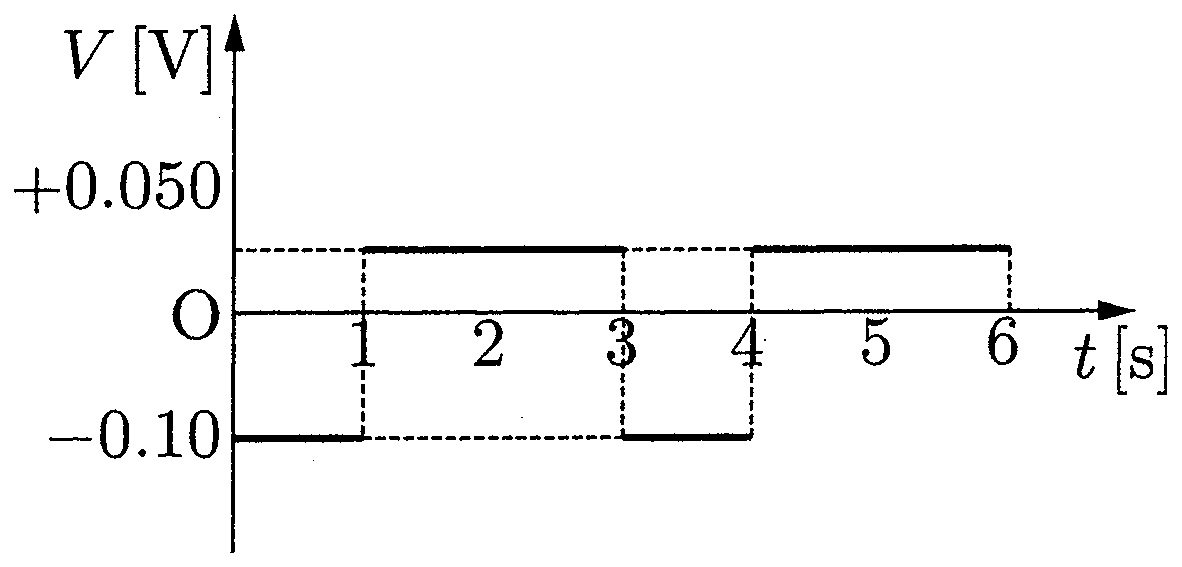
\includegraphics[keepaspectratio,width=52mm]{fig/n30_a105_graph.png}\end{center}
\begin{chuu}
誘導起電力の向きを考える際に，誘導電流といったものを考えるが，実際に流れ続けているわけではないことに注意せよ．本問のように二次コイルが閉ループをつくっておらず，開いている場合には，誘導電流は流れ続けることができず，コイルの両端に相互誘導起電力による電位差のみが発生することになる．
\end{chuu}

\MonN{106}{変圧器}\par\nopagebreak
\begin{sisin}
交流電圧の大きさを変換するのに利用される装置がこの変圧器である（30.5）．本問のように時間変動する電流を流すと相互誘導により二次コイル側に時間変動する電圧が現れることを利用している．前問と全く同様に相互誘導起電力を考えよう．一次コイル側の電流$I_1$により生じる磁束は，鉄心によりねじ曲げられて二次コイルを貫くことに注意せよ．
\end{sisin}
\KaiHead
今，コイル1に電流$I_1$が流れると，コイル1を下向きに貫く磁束が鉄心内に発生する．この磁束は鉄心によりねじ曲げられて，コイル2を上向きに貫く（次図参照）．
\begin{center}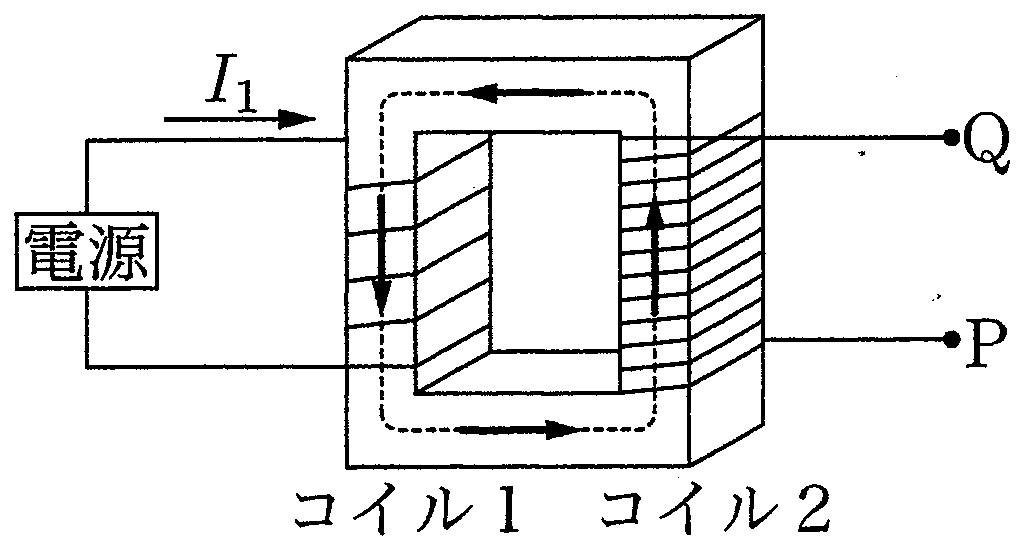
\includegraphics[keepaspectratio,width=48mm]{fig/n30_a106_zu.png}\end{center}
この磁束と同じ向きの磁場をコイル2が発生するためには電流が$\mathrm{P}\to\mathrm{Q}$に流れればよく，この向きが電流の正の向きである．コイル2内をこの向きに誘導電流が流れると，$\mathrm{P}$の方が高電位になるので，$\mathrm{Q}$が高電位の向きを正とした相互誘導起電力は，
\[V=-M\frac{dI_1}{dt}=-0.50\frac{dI_1}{dt}\U{V}\]
と表される．図2から電流の時間変化率を求めると，
\[\frac{dI_1}{dt}=\left\{\begin{aligned}
  &+15\U{A/s}\quad(0<t<0.02)\\
  &+5.0\U{A/s}\quad(0.02<t<0.06)\\
  &\ 0\U{A/s}\quad(0.06<t<0.12)\\
  &-10\U{A/s}\quad(0.12<t<0.17)
\end{aligned}\right.\]
であるから，求めるグラフは次図のようになる．\Ans
\begin{center}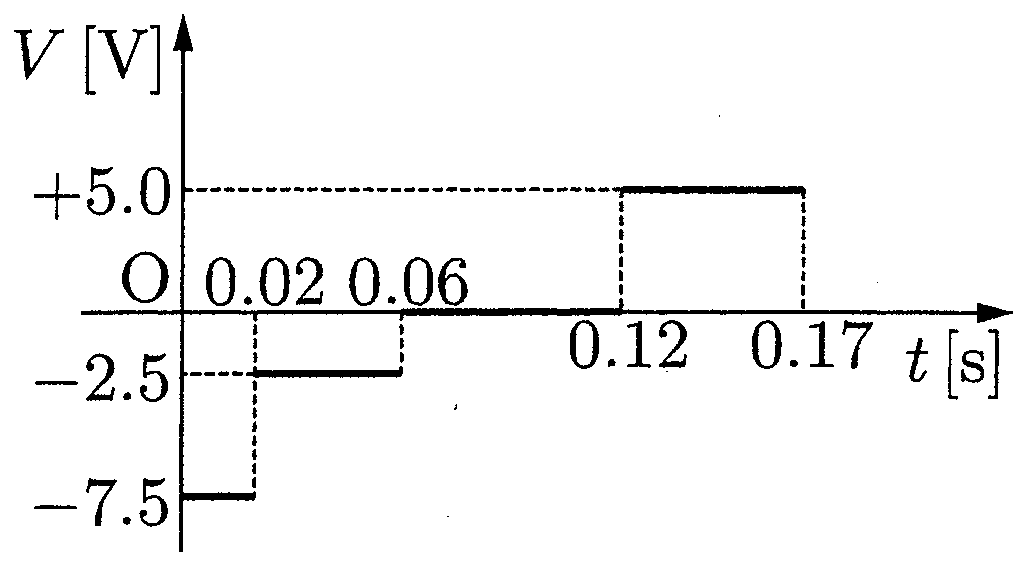
\includegraphics[keepaspectratio,width=50mm]{fig/n30_a106_graph.png}\end{center}

\MonN{107}{相互インダクタンスの計算}\par\nopagebreak
\begin{sisin}
自己・相互インダクタンスを求めるためには，\MARU{1}一次コイル側に流れる電流がつくる磁場・磁束を求める，\MARU{2}電流変化により生じる誘導起電力を求める，\MARU{3}比例定数部分を取って自己インダクタンス，相互インダクタンスを求める，という流れで考えよ（例題33）．

ソレノイドコイルの磁場の強さは$H=n_0I$であるが，$n_0$は{\gtfamily 単位長さあたりの}巻き数であることに注意．一方，誘導起電力の大きさは1ループあたり$\dfrac{d\varPhi}{dt}$であり，$N$回巻きのコイルなら$N\dfrac{d\varPhi}{dt}$である．{\gtfamily $N$倍するのを忘れないようにせよ．}
\end{sisin}
\KaiHead
ソレノイドコイル$\mathrm{P}$を一次コイルとみなし，$\mathrm{a}\to\mathrm{b}$向きの電流$I$を流した場合について考えると，コイル$\mathrm{P}$内には右ねじの法則より，左向きに一様な磁場が発生し，その強さは$H=\dfrac{N_1}{l_1}I$となる．この磁場はコイルの断面に対して垂直であるから，コイル$\mathrm{P}$，$\mathrm{Q}$を貫く磁束は，
\[\varPhi_{\mathrm{P}}=\frac{\mu_0N_1S_1}{l_1}I,\qquad\varPhi_{\mathrm{Q}}=\frac{\mu_0N_1S_2}{l_1}I\]
である．
\begin{komon}
\ko{1} 一次コイル$\mathrm{P}$に発生する誘導起電力を$V_{\mathrm{P}}$とすると，ファラデーの電磁誘導の法則より，
       \[V_{\mathrm{P}}=-N_1\frac{d\varPhi_{\mathrm{P}}}{dt}=-\frac{\mu_0N_1^2S_1}{l_1}\cdot\frac{dI}{dt}\]
       以上より自己インダクタンスは，
       \[L=\frac{\mu_0N_1^2S_1}{l_1}\U{H}\Ans\]
\ko{2} 二次コイル$\mathrm{Q}$の巻き方から考えて$\mathrm{Q}$内を$\mathrm{c}\to\mathrm{d}$の向きに電流が流れるときが正であり，二次コイル$\mathrm{Q}$で発生する誘導起電力を$V_{\mathrm{Q}}$とすると，巻き数が$N_2$であることに注意して，
       \[V_{\mathrm{Q}}=-N_2\frac{d\varPhi_{\mathrm{Q}}}{dt}=-\frac{\mu_0N_1N_2S_2}{l_1}\cdot\frac{dI}{dt}\]
       以上より相互インダクタンスは，
       \[M=\frac{\mu_0N_1N_2S_2}{l_1}\U{H}\Ans\]
\end{komon}
\begin{bsHosoku}{参考}
上述した解答では，一次コイルの電流変化により生じる誘導起電力を求め，比例定数部をインダクタンスと置く方法で求めたが，実は自己インダクタンスと相互インダクタンスには，
\[N_1\varPhi_{\mathrm{P}}=LI,\qquad N_2\varPhi_{\mathrm{Q}}=MI_1\]
という性質があり，これらを用いて自己・相互インダクタンスを求めることも可能である．$-N_1\dfrac{d\varPhi_{\mathrm{P}}}{dt}=-L\dfrac{dI}{dt}$の両辺を$t$で積分し，$I=0$のとき$\varPhi_{\mathrm{P}}=0$であることを使えば示せる（相互インダクタンスも同様）．逆に，コイルの自己インダクタンスが与えられていれば，これらの式を用いて，コイルを貫く磁束を計算することができる．
\end{bsHosoku}

\MonN{108}{相互インダクタンス}\par\nopagebreak
\begin{sisin}
［107］と同じ流れ（磁場 → 磁束 → 誘導起電力 → 比例定数）で考える．$R\gg r$なので，小さいコイル$\mathrm{B}$の範囲では$\mathrm{A}$のつくる磁場は中心の値で一様とみなしてよい．$\mathrm{B}$は$n$回巻きなので，誘導起電力は1巻きあたりの$n$倍になる．
% 原本の例題38．原本には解答が無いので書き起こした．
\end{sisin}
\KaiHead
\begin{komon}
\ko{1} $N$回巻きの円形電流の中心の磁場なので，
       \[H=\frac{NI}{2R}\U{A/m}\Ans\]
\ko{2} $\mathrm{B}$の範囲の磁束密度は$\mu_0H$で一様とみなせるので，1巻きを貫く磁束は
       \[\varPhi=\mu_0\frac{NI}{2R}\cdot\pi r^2=\frac{\pi\mu_0Nr^2}{2R}I\U{Wb}\Ans\]
\ko{3} $\varDelta\varPhi=\dfrac{\pi\mu_0Nr^2}{2R}\varDelta I$で，$\mathrm{B}$は$n$回巻きなので
       \[V=n\frac{\varDelta\varPhi}{\varDelta t}=\frac{\pi\mu_0Nnr^2}{2R}\cdot\frac{\varDelta I}{\varDelta t}\U{V}\Ans\]
\ko{4} $V=M\dfrac{\varDelta I}{\varDelta t}$と比べて，
       \[M=\frac{\pi\mu_0Nnr^2}{2R}\U{H}\Ans\]
       （［107］の参考の$n\varPhi=MI$からも直ちに求まる．）
\end{komon}

\Rank{C問題}
\MonN{109}{誘導電場}\par\nopagebreak
\begin{sisin}
誘導起電力の発生の原因を考える問題である（30.2）．［102］のように考えると，回路が磁場を横切っていかない限りは誘導起電力が発生しないことになるが，一般に，時間的に変化する磁場のまわりには誘導電場と呼ばれる電場が発生する．変化する磁場のまわりの半径$R$の円周上に誘導起電力が発生するのはこの誘導電場のせいであるが，問題後半にもあるように，誘導電場はその位置にループがなくても空間中に発生できるため，このことを利用すると本問のように磁場の変化によって粒子を加速することができる．この原理はベータトロンと呼ばれる電子の加速装置などに利用されている．
\end{sisin}
\KaiHead
\begin{komon}
\ko{1} 円の面積は$S=\pi R^2$であり，ループを貫く磁束を$\varPhi=BS$として，ファラデーの電磁誘導の法則より，
       \[V=\left|-\frac{d\varPhi}{dt}\right|=S\frac{dB}{dt}=\pi R^2\frac{dB}{dt}\U{V}\Ans\]
\ko{2} $V=E\cdot 2\pi R$の関係式より，
       \[E=\frac{V}{2\pi R}=\frac{R}{2}\cdot\frac{dB}{dt}\U{V/m}\Ans\]
\ko{3} 上向きの磁束が増加するので，このループに発生する誘導電流の向きはレンツの法則より時計回りの向きであり，この向きに電流を流そうとする誘導起電力が発生する．よって，この導線上の正電荷は時計回りに力を受ける．これは，この向きに誘導電場が発生していることを意味する．以上より，誘導電場の向きは{\gtfamily 時計回り}．\Ans
       \begin{center}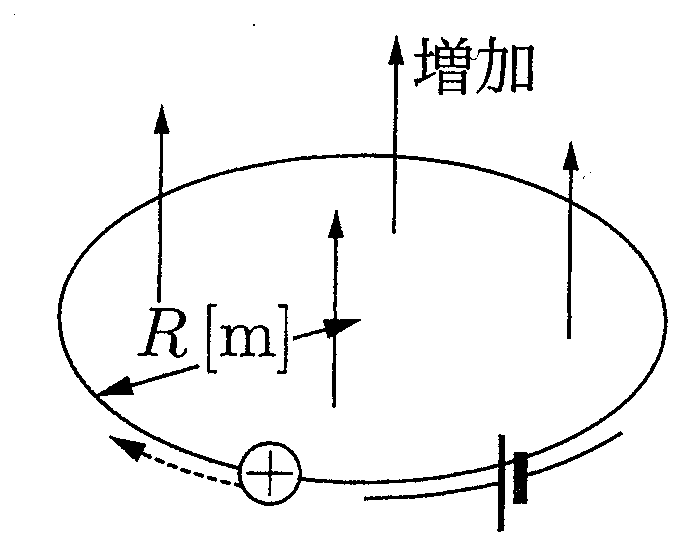
\includegraphics[keepaspectratio,width=36mm]{fig/n30_a109_zu.png}\end{center}
\ko{4} 円環上には$E=\dfrac{R}{2}\cdot\dfrac{dB}{dt}$の誘導電場が発生する．よって，この粒子の加速度$a$は運動方程式$ma=qE$より，
       % 原本は左辺が「q=」になっていた（誤植）．
       \[a=\frac{qR}{2m}\cdot\frac{dB}{dt}\U{m/s^2}\Ans\]
\end{komon}

\MonN{110}{相互誘導起電力}\par\nopagebreak
\begin{sisin}
$\mathrm{L}$が振れるのは$\mathrm{L}$に対して電磁力が作用するためであるが，ソレノイドコイルがつくる磁場から$\mathrm{L}$が電磁力を受けると考えてしまうと考えにくい．本問では力の作用する向きのみを判断すればよいので，コイル$\mathrm{AB}$とコイル$\mathrm{L}$とが平行電流になっていることに着目して，同じ向きの平行電流であれば引力，逆向きの平行電流なら斥力を作用しあうことを利用しよう（第28回）．

なお，コイル$\mathrm{AB}$には自己インダクタンスがあるので，スイッチを入れてもいきなり電流が$\dfrac{E}{R}$にはならず，次第に増加して$\dfrac{E}{R}$になる（第31回で詳しく学ぶ）．
% 原本は「B問題［25］と同様」（旧回の番号）．
\end{sisin}
\KaiHead
\begin{komon}
\ko{1} スイッチを閉じることによりソレノイドコイル$\mathrm{AB}$に電流が流れると，次図のような磁場が発生する（ソレノイドコイル両端からは磁場が広がるように出ていく）．
       \begin{center}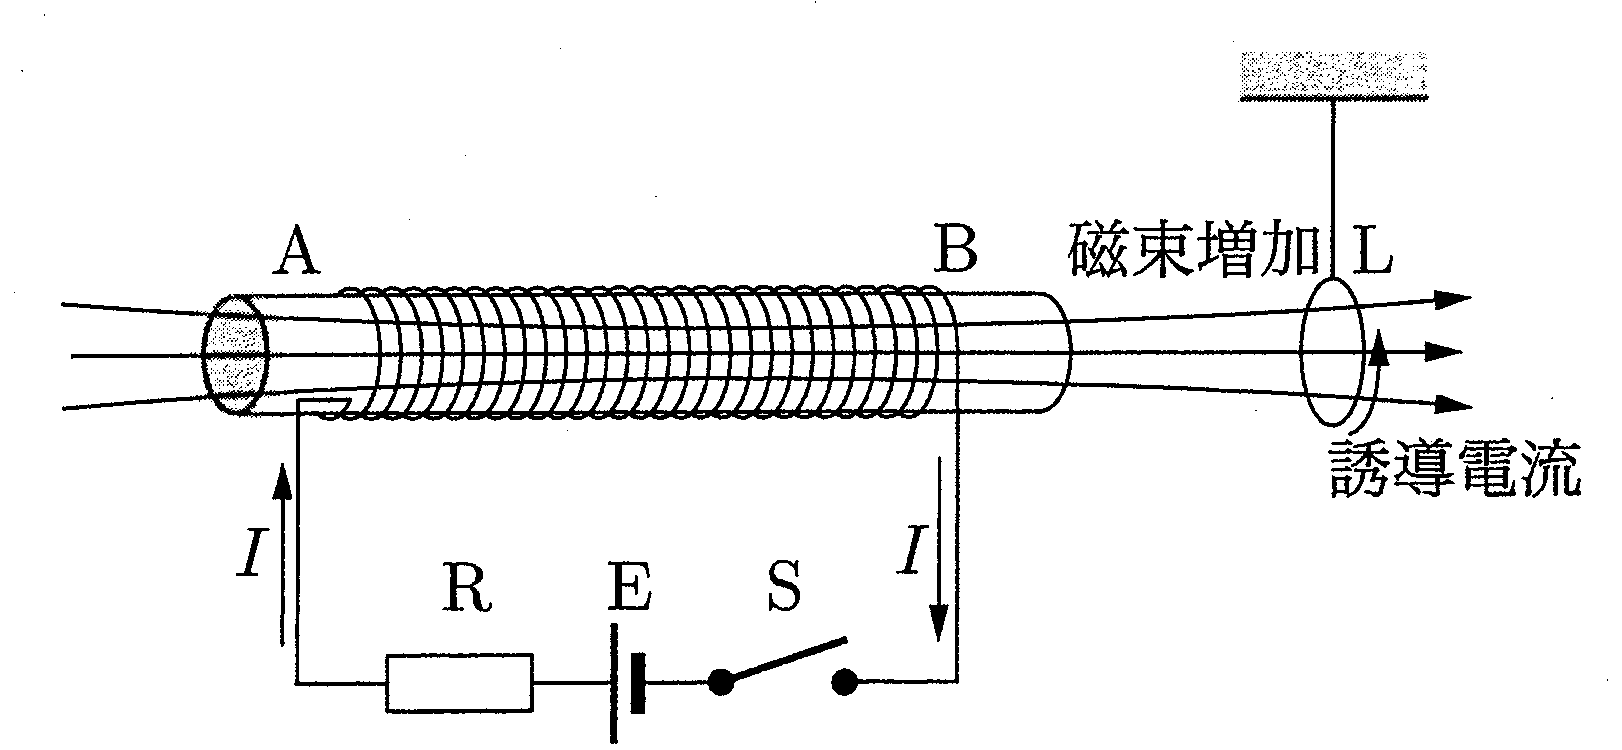
\includegraphics[keepaspectratio,width=60mm]{fig/n30_a110_zu1.png}\end{center}
       コイル$\mathrm{AB}$に流れる電流$I$が次第に増加していくと，コイル$\mathrm{L}$を右向きに貫く磁束が増加していくので，レンツの法則よりコイル$\mathrm{AB}$から見て{\gtfamily 反時計回り}に誘導電流が流れる．\Ans
\ko{2} またこの電流の向きは，前図より$I$と{\gtfamily 逆}向きである．\Ans
\ko{3} コイル$\mathrm{AB}$の導線とコイル$\mathrm{L}$の導線は平行導線とみなせる．(2)より，この平行導線には逆向きに電流が流れているので，互いに斥力を及ぼし合う．よって，$\mathrm{L}$は$\mathrm{AB}$に{\gtfamily 反発さ}れる．\Ans
\ko{4} スイッチ$\mathrm{S}$を切ると，コイル$\mathrm{AB}$に流れる電流$I$が減少するので，コイル$\mathrm{L}$を右向きに貫く磁束が減少することになる．よって，コイル$\mathrm{L}$には$\mathrm{AB}$側から見て時計回りに誘導電流が流れることになり，これはコイル$\mathrm{AB}$に流れる電流と互いに同じ向きの平行電流になっている．よって，$\mathrm{L}$は$\mathrm{AB}$に{\gtfamily 引き付けら}れる．\Ans
\end{komon}
\begin{bsHosoku}{参考}
平行電流間に作用する力の考え方を利用したが，ソレノイドコイルのつくる磁場から受ける電磁力として判断することもできる．コイル端からはみ出した磁場は(1)で示したように広がっていき，コイル$\mathrm{L}$の導線部分に対しては多少斜めに磁場がかかっている．$\mathrm{L}$を微小部分に分け，任意の微小部分$\mathrm{P}$と，中心軸に対して対称な微小部分$\mathrm{Q}$が受ける力を考えると，次図のようになる．
\begin{center}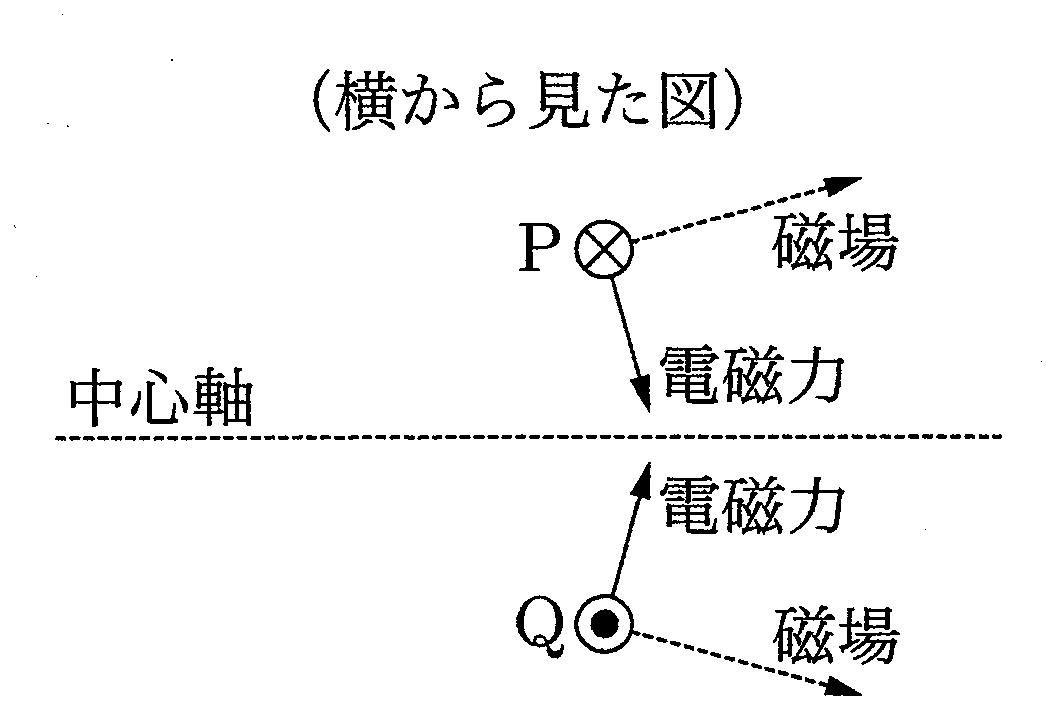
\includegraphics[keepaspectratio,width=40mm]{fig/n30_a110_zu2.png}\end{center}
$\mathrm{P}$，$\mathrm{Q}$が受ける力を合成すると左→右向き（斥力）となり，$\mathrm{L}$全体が受ける力は斥力となる．(4)についても同様な考え方で受ける力を求めることができる．
\end{bsHosoku}

\end{multicols}
